\documentclass[10pt]{scrreprt}
\usepackage[a4paper, top=30mm, left=25mm, right=25mm, bottom=30mm]{geometry}
\usepackage[utf8]{inputenc}

\usepackage[Bjornstrup]{fncychap}
\usepackage{ngerman}
\usepackage{graphicx}
\usepackage{epstopdf}
\usepackage{etoolbox}
\usepackage{enumitem}
\usepackage{url}
\usepackage{numprint}
\usepackage{longtable}
\usepackage{tabu}
\usepackage{multirow}
\usepackage{caption}
\usepackage{array}
\usepackage{amssymb}


\makeatletter
\patchcmd{\@makechapterhead}{\vspace*{50\p@}}{\vspace*{-20\p@}}{}{}
\patchcmd{\@makeschapterhead}{\vspace*{50\p@}}{\vspace*{7\p@}}{}{}
\patchcmd{\DOTIS}{\vskip 40\p@}{\vskip -12\p@} 
\makeatother
  
\captionsetup[figure]{labelfont={sf,bf},textfont={sf}}
\deffootnotemark{[\thefootnotemark]}
\deffootnote{1.5em}{1em}{[\thefootnotemark] }
\setlength{\parindent}{0pt}
\renewcommand{\labelitemi}{ \raisebox{0.3ex}{\small$\blacktriangleright$} }

\newcommand{\sfbf}[1]{\textbf{\sffamily #1}}
\newcommand{\sfit}[1]{\textit{\sffamily #1}}
\newcommand{\W}{\sfbf{W}}
\newcommand{\ziel}[1]{{\fontsize{9.5}{11}\textsf{/#1/}}}
\newcommand{\ziellabel}{Z}
\newcommand{\muss}{\renewcommand{\labelenumi}{\textbf{\ziel{\ziellabel\numprint{\theenumi}0}}}}
\newcommand{\wunsch}{\renewcommand{\labelenumi}{\textbf{\ziel{\ziellabel\numprint{\theenumi}0W}}}}
\newcommand{\JoglEarth}{\raisebox{-1.2mm}{
\includegraphics[scale=0.33]{Logo-Text.eps}} }
\newcommand{\textref}[1]{\mbox{\raisebox{0.1ex}{\small$\rightarrow$ }\textit{#1}}}

\newenvironment{details}[1][6pt]{%
  \parskip#1 \parindent6mm \raggedright%
  \def\item{\par\ignorespaces\hangindent=5mm \hangafter1}}{%
  \par\ignorespaces} 
  

\begin{document}

\thispagestyle{empty}
\sffamily
 
\title{Pflichtenheft}

\begin{figure}
\begin{flushright}
	
\includegraphics[scale=0.4]{uniLogo.eps}
\vspace{2.0 cm}
\end{flushright}
\end{figure}

\begin{center}
\vspace{2.0 cm}
{\LARGE SEP – Wintersemester 2013/14}

\vspace{1.0 cm}
\textbf{{\Huge Pflichtenheft}}

\vspace{0.8 cm}
\begin{figure}[!htb]
\begin{center}
	%
\includegraphics[scale=1.0]{projektLogo.eps}
	
\includegraphics[scale=1.5]{Logo-Print.eps}
\end{center}
\end{figure}

\vspace{0.2 cm}
\textbf{{\huge OpenStreetMap: Die Welt in 3D}}

\vspace{1.5 cm}
31.10.2013

\vspace{0.5 cm}
Version: 1.1

\vspace{1.5 cm}
{\Large Projektbetreuer: Peter Barth}

\vspace{1.5 cm}
\begin{tabular}{|c|c|c|}
\hline 
\rule[-1ex]{0pt}{4ex} \textbf{Phase} & \textbf{Verantwortlicher} & \textbf{E-Mail Adresse} \\ 
\hline  \hline
\rule[-1ex]{0pt}{4ex} Pflichtenheft & Gabriele Haas & haasgab@fim.uni-passau.de \\ 
\hline  \hline
\rule[-1ex]{0pt}{4ex} Entwurf & Thomas Eder & ederthom@fim.uni-passau.de \\ 
\hline  \hline
\rule[-1ex]{0pt}{4ex} Spezifikation & Christof Blauberger & blauberg@fim.uni-passau.de \\ 
\hline  \hline
\rule[-1ex]{0pt}{4ex} Implementierung & Fabian Knorr & knorrfab@fim.uni-passau.de \\ 
\hline \hline 
\rule[-1ex]{0pt}{4ex} Testing & Constantin Wenger & wengerco@fim.uni-passau.de \\ 
\hline  \hline
\rule[-1ex]{0pt}{4ex} Präsentation & Sebastian Reichl & reichlse@fim.uni-passau.de \\ 
\hline 
\end{tabular}

\end{center}


\pagebreak
\rmfamily
\tableofcontents


\chapter{Ausgangssituation}
Die Karten des OpenStreetMap-Projekts erfreuen sich immer größerer Beliebtheit. Der Detailgrad, die Menge an verschiedenen Merkmalen und die Genauigkeit der Daten sind die ihrer Konkurrenz in den meisten Regionen der Welt weit voraus. Durch die große Auswahl an Informationen und die Flexibilität in der Darstellung eröffnen sich unzählige Anwendungsmöglichkeiten.

Die Grafikleistung einfacher Desktoprechner ist bereits für aufwändige 3D-Szenarien ausgelegt. Die Ansprüche der Benutzer hat sich in den letzten Jahren dahingehend geändert, dass ansprechende visuelle Gestaltung und einfache Bedienung ausschlaggebend für die Wahl eines Softwareproduktes ist.

\vspace{0.5cm}

Die Projektion einer Straßenkarte auf einen dreidimensionalen Globus ist die intuitivste und geographisch korrekteste Darstellung. Es liegt also nahe, auf dieser Grundlage eine Anwendung zur Kartenanzeige zu entwickeln.

Da bereits Projekte mit einem gleichen oder ähnlichen Ziel existieren, möchten wir uns von diesen durch die folgenden Schwerpunkte abgrenzen:
\begin{itemize}
\item Verwendung der freien Kartendaten des OpenStreetMap-Projekts
\item Realisierung einer dreidimensionalen Globusoberfläche mit den Höhendaten der NASA
\item Intuitive Bedienung der Anwendung ohne Einarbeitungszeit
\item Die Möglichkeit der spielerischen Benutzung durch Kinder ohne nennenswerte PC-Kenntnisse
\item Vollständige Plattformunabhängigkeit durch Java
\item Effiziente Speicher- und Bandbreitennutzung
\end{itemize}

\vspace{0.5cm}

Basierend auf diesen Grundprinzipien wird in diesem Pflichenheft das Konzept der Desktopanwendung \JoglEarth entwickelt.




\chapter{Produkteinsatz}
\section{Anwendungsbereich}
\JoglEarth soll eine dreidimensionale Ansicht der Welt sowie eine ebene Kartenansicht bieten. Beides erfolgt auf Basis des OpenStreetMap-Projekts und Satellitendaten der NASA. \\

Die grafische Benutzeroberfläche zeigt dafür im dreidimensionalen Modus eine Weltkugel, die frei gedreht und gezoomt werden kann, und im zweidimensionalen einen Ausschnitt der Weltkarte. Die Karte kann aus verschiedenen Kategorien wie Satellitenbildern oder Straßenkarten gewählt werden. Die Steuerung erfolgt mit Tastatur und Maus. \\

Mit einer Suchfunktion kann im Umkreis oder global nach Orten gesucht werden. Punkte besonderen Interesses wie Tankstellen oder Banken können über dem Kartenbild eingeblendet werden.

\section{Zielgruppe}
Primäre Zielgruppe des Systems sind Privatanwender, die eine andere Art der Kartendarstellung als die typischen Onlinekarten bevorzugen. \\

Auch soll die Anwendung wissbegierige Kinder ansprechen. Voraussetzung ist lediglich der geübte Umgang mit der Maus und/ oder Tastatur.


\section{Sicherheit, Datenschutz}
Die Anwendung wahrt von vorne herein die Sicherheit des Systems und schützt die Privatsphäre des Nutzers. Da sie keine sicherheitskritischen Daten verarbeiten muss, ist dies implizit gegeben und stellt keine besondere Anforderung an den Entwurf dar.
\begin{itemize}
\item Es ist weder zur Bedienung, noch zum Beschaffen der Kartendaten eine Authentifikation erforderlich 
\item Es werden keine persönlichen Daten des Anwenders über das Netz übertragen
\item Es wird kein Code aus dem Netz nachgeladen und ausgeführt
\item Das Programm hat keine (unter Umständen angreifbare) Serverfunktionalität
\end{itemize}

\pagebreak
\section{Lizenzen}
Wird das Produkt veröffentlicht, so müssen die Lizenzen der verwendeten Bibliotheken und Datenquellen berücksichtigt werden:
\begin{itemize}
\item Die Teile der JOGL-Bibliothek sind unter mehreren Versionen der BSD-Lizenz, der SGI Free Software License und der Apache-Lizenz, der Ubuntu Font License und mehreren proprietären Lizenzen veröffentlicht. Details dazu finden sich bei  \footnote{\url{https://jogamp.org/git/?p=jogl.git;a=blob;f=LICENSE.txt}}.
\item OpenStreetMap ist „OpenData“ im Sinne der Open Database Lizenz (ODbL). Die Kartenkacheln stehen unter der Linzenz  Creative Commons „Namensnennung, Weitergabe unter gleichen Bedingungen" 2.0 (CC BY-SA). Weitere Infos, wie auch eine Vorgabe zum Hinweisen auf der Urheberschaft des OSM-Projekts finden sich bei \footnote{\url{http://www.openstretmap.org/copyright}}.
\item Die Daten der Overpass API sowie Nominatim stehen ebenfalls unter der ODbL.
\item Die Satellitenbilder der NASA sind für die Zwecke des Projekts frei verfügbar und stehen unter der Lizenz, die sich bei \footnote{\url{http://www.nasa.gov/audience/formedia/features/MP_Photo_Guidelines.html}} findet.
\item Die Verwendete GUI-Bibliothek JGoodies Forms steht unter der BSD-Lizenz bei \footnote{\url{http://opensource.org/licenses/bsd-license.html}}.
\end{itemize}




\chapter{Produktumgebung}
\section{Software}
Da das Projekt auf Java setzt, ist es betriebssystemunabhängig. Es muss lediglich das Java Runtime Environment (JRE) in Version 7 sowie ein Fenstersystem und Netzwerkunterstützung zur Verfügung stehen. Um das Handbuch über die Hilfefunktion anzeigen zu können, muss auf dem System außerdem ein PDF-Betrachter installiert sein. Zusätzliche Programmbibliotheken, die zum Ausführen des Softwarepakets nötig sind, werden mitgeliefert.\\

Da die Software von Seiten der Entwickler nur auf einem kleinen Teil der möglichen Umgebungen getestet werden kann, sollen mindestens folgende Konfigurationen unterstützt werden:
\begin{itemize}
\item Windows 7 und 8 auf x86{\_}64 mit den Herstellertreibern von nVidia und AMD
\item Linux auf x86{\_}64 mit X.org und proprietären Treibern von nVidia / AMD sowie den freien radeon-Treibern für AMD
\end{itemize}


\section{Hardware}
Wie schon bei der Software der Fall sollte die Anwendung auch mit nahezu allen modernen Desktopsystemen kompatibel sein. Folgende (oder eine gleichwertige) Konfiguration wird jedoch für ein optimales Benutzererlebnis mindestens empfohlen:
\begin{itemize}
\item Dual-Core-Prozessor mit 1 GHz Taktfrequenz
\item 2 Gigabyte RAM
\item 200 Megabyte freier Speicherplatz
\item Grafikkarte: Onboard-Grafik mit OpenGL 2.0-Unterstützung
\item Bildschirm mit 1024x768 Pixeln Auflösung und 24 Bit Farbtiefe
\item Standard-Tastatur und Maus
\end{itemize}



\section{Orgware}
Zum Laden der Kartendaten wird eine durchgehende Internetverbindung benötigt. Um die Wartezeiten akzeptabel zu halten wird mindestens 1MBit/s empfohlen.




\chapter{Zielbestimmungen}

\section{Musskriterien}
\begin{itemize}
\item Grafisch ansprechende GUI mit einklappbarer Seitenleiste und\\ Sprachunterstützung für Englisch und Deutsch (\ziel{F010} - \ziel{F040})
\item Mit OpenGL gerenderte Kartenansicht, die mit Maus und Tastatur intuitiv bedienbar ist (\ziel{F190}, \ziel{F200}, \ziel{F260}, \ziel{F280}, \ziel{F290}, \ziel{F550})
\item Anzeige der momentanen und möglichen Zoomstufen (\ziel{F050}, \ziel{F060})
\item Sinnvolle Beschränkung von Zoom und Beweglichkeit (\ziel{F420}, \ziel{F430}, \ziel{F450} - \ziel{F470})
\item Ladebalken für im Hintergrund geladene Kartendaten (\ziel{F070})
\item Felder zur Anzeige und Änderung des Längen- und Breitengrads (\ziel{F080}, \ziel{F090}, \ziel{F230}, \ziel{F390})
\item Wechselmöglichkeit zwischen Globus- und flacher Kartenansicht (\ziel{F300})
\item Wechselmöglichkeit zwischen Satellitenbildern und OpenStreetMap-Karten (\ziel{F310})
\item Drehen, Kippen, Zoomen der Ansichten (\ziel{F410} - \ziel{F470})
\item Text- und Symboloverlays für Städte und POIs, Anzeige der Details dazu im Detailfenster\\(ohne Markierung und Speicherfunktion)(\ziel{F140}, \ziel{F150}, \ziel{F240}, \ziel{F360}, \ziel{F480}, \ziel{580})
\item Beschränkung der Anzahl gleichzeitig geladener Overpass-Einträge zur Ressourcenschonung \\(siehe \ziel{F480})
\item Effizientes, asynchrones Laden von Daten durch Caching (\ziel{F510} - \ziel{F540}, \ziel{F620})
\item Sternenhimmel als Hintergrund (\ziel{F380})
\item Anzeige des Benutzerhandbuchs und eines Infofensters (\ziel{F100}, \ziel{F110})
\item Speichern und Laden von Einstellungen (\ziel{F600}, \ziel{F610})
\item Verwendung einer Platzhaltertextur für nicht verfügbare Kacheln
\end{itemize}

\section{Wunschkriterien}
\begin{itemize}
\item Kinder-Weltkarte als zusätzliche Kartenoption (\ziel{F310})
\item Sonnensystem-Modellansicht als weiteren Ansichtsmodus (\ziel{F300})
\item Anzeige des momentanen Kartenmaßstabs (\ziel{F250W})
\item Dreidimensionales Höhenprofil auf Globus- und Kartenoberfläche (\ziel{F210W}, \ziel{F220W}, \ziel{F320W}, \ziel{F560W})
\item Änderung des Detailgrads des 3D-Modells (siehe \ziel{F330W})
\item Funktion zum Markieren und Speichern von Punkten (\ziel{F120W}, \ziel{F130W}, \ziel{F230}, \ziel{F370W}, \ziel{F490W}, \ziel{F500W})
\item Anzeige von Informationen zum Bildmittelpunkt (\ziel{F570W})
\item Lokale und Globale Suchfunktion (\ziel{F160W} - \ziel{F180W}, \ziel{F590W})
\item Zusätzliche Grafikeinstellungen wie Antialiasing oder Texturfilterung (\ziel{F330W} - \ziel{F350W})
\item Vorausladen von Kartendaten an den Rändern der Anzeige und die der nächsten Zoomstufen (\ziel{F270})
\item Aussetzen des Renderns bis zur Bildänderung 
\end{itemize}

\section{Abgrenzungskriterien}
\begin{itemize}
\item Keine Druck- oder Speicherfunktion für Kartenmaterial
\item Keine Exportfunktion für markierte Punkte (Speicherfunktion in externe Datei)
\item Keine dynamischen Flüsse oder andere Animationen
\item Keine 3D-Modelle für Häuser, Bäume oder Ähnliches
\item Keine Routenplanung
\item Keine Unterstützung für andere als die angegebenen Eingabegeräte
\item Keine Authentifizierung um Zugriff auf vom Benutzer gespeicherte Markierungen zu erhalten
\item Keine Kollisionserkennung bei Höhenprofilen
\end{itemize}


\chapter{Benutzeroberfläche}

\section{Visuelles Konzept}

\begin{itemize}
	\item Das Hauptelement der Benutzeroberfläche ist das \textit{Ansichtsfenster} \raisebox{-1pt}{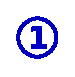
\includegraphics[scale=0.45]{Nummern/1.eps}}, das sich in der Fenstermitte befindet. In ihm wird der Globus, die Kartenebene oder eine Sonnensystemansicht angezeigt. Der sichtbare Kartenausschnitt kann interaktiv mit Maus oder Tastatur verschoben, gedreht gezoomt und gekippt werden.
	\item Am linken Rand des Fensters befindet sich die \textit{Seitenleiste} \raisebox{-1pt}{
\includegraphics[scale=0.45]{Nummern/2.eps}}, die die meisten Steuerungsoptionen bereitstellt. Der obere Teil ist in Tabs unterteilt, mit denen Funktionen gruppiert werden; der untere Teil zeigt Details zum momentan zentrierten Punkt an. Um den sichtbaren Kartenbereich zu vergrößern, ist sie ausblendbar.
	\item Am rechten Rand \raisebox{-1pt}{
\includegraphics[scale=0.45]{Nummern/3.eps}} befindet sich ein Schieber, mit dem das Zoomlevel angezeigt und geändert werden kann.
	\item Die \textit{Statusleiste} \raisebox{-1pt}{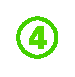
\includegraphics[scale=0.45]{Nummern/4.eps}} am unteren Rand beinhaltet Informationen über den zentrierten Punkt, wie Koordinaten und Maßstab. Außerdem wird in ihm der Fortschritt im Hintergrund geladener Daten angezeigt.
\end{itemize}


\vspace{1cm}
\begin{figure}[h]
	\centering
	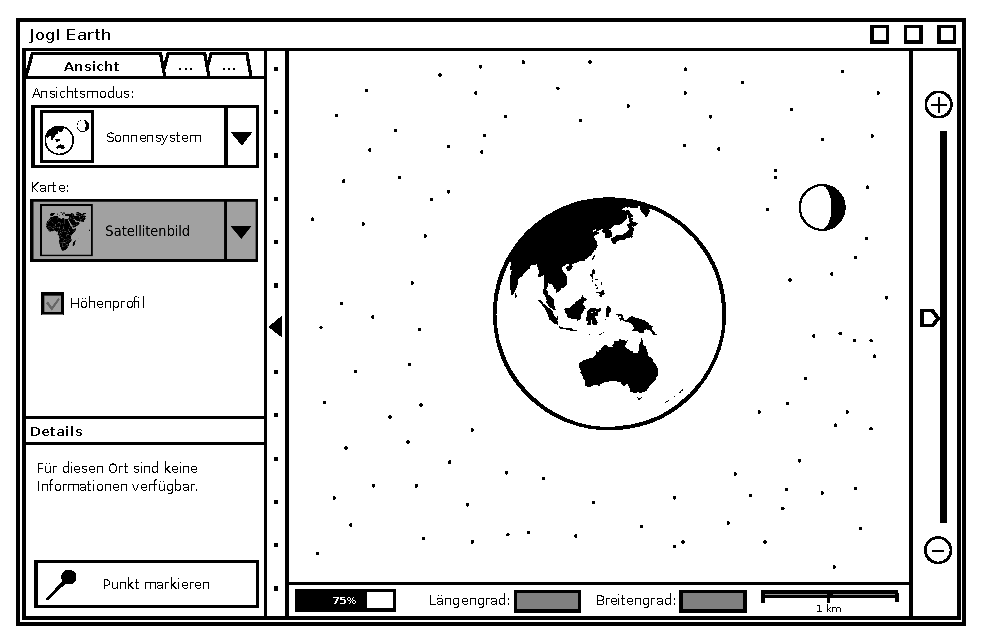
\includegraphics[scale=0.9]{GUI-Sonnensystem.eps}
	\caption{Die Benutzeroberfläche mit geöffnetem Ansichts-Tab im Sonnensystemmodus}
\end{figure}

\begin{figure}
	\centering
	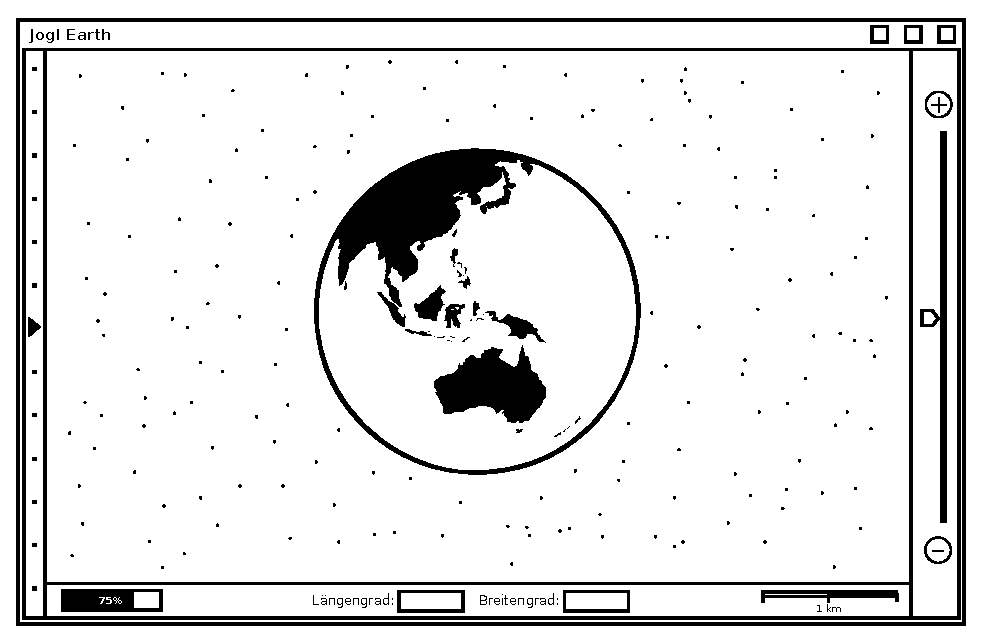
\includegraphics[scale=0.9]{GUI-Ausgeblendet.eps}
	\caption{Die Benutzeroberfläche mit ausgeblendeter Einstellungsleiste und dargestelltem Globus}
\end{figure}

\begin{figure}
	\centering
	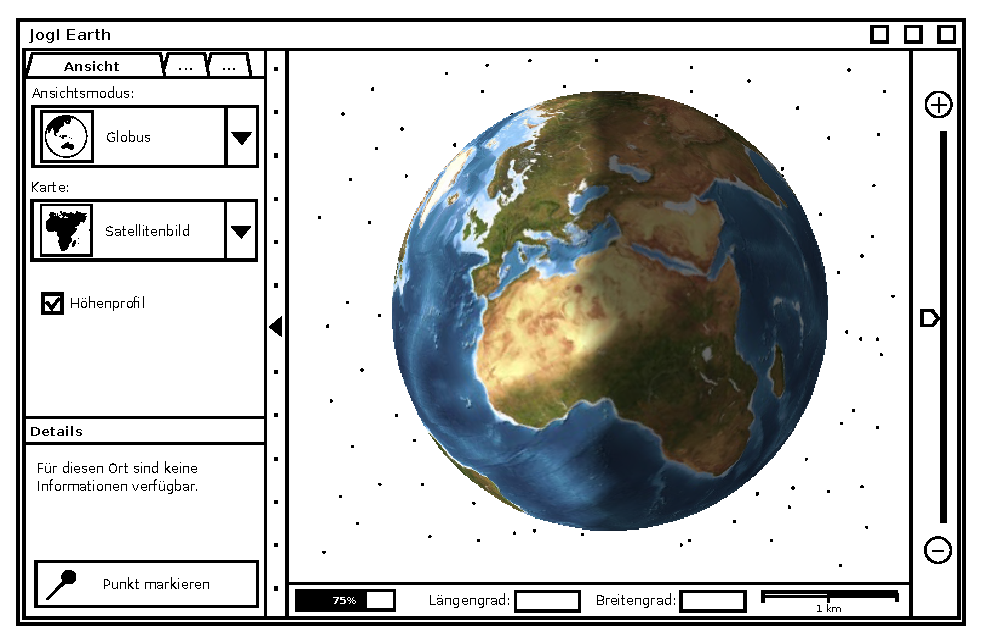
\includegraphics[scale=0.9]{GUI-Ansicht-Welt.eps}
	\caption{Die Benutzeroberfläche mit gewählter Satellitenansicht}
\end{figure}
\begin{figure}
	\centering
	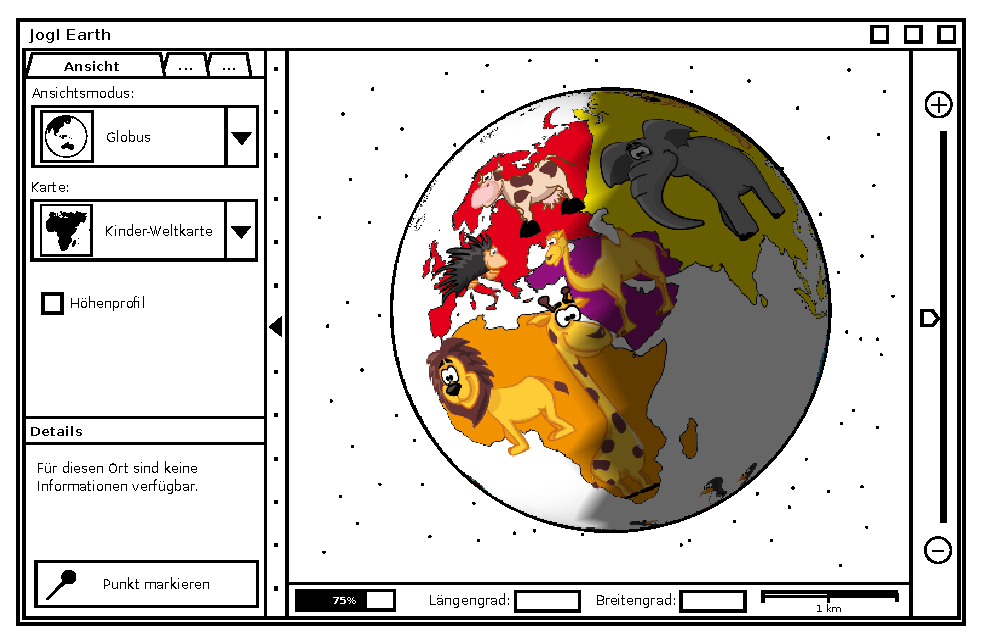
\includegraphics[scale=0.9]{GUI-Ansicht-Kinder-Weltkarte.eps}
	\caption{Die Benutzeroberfläche mit gewählter Kinder-Weltkarte}
\end{figure}
\begin{figure}
	\centering
	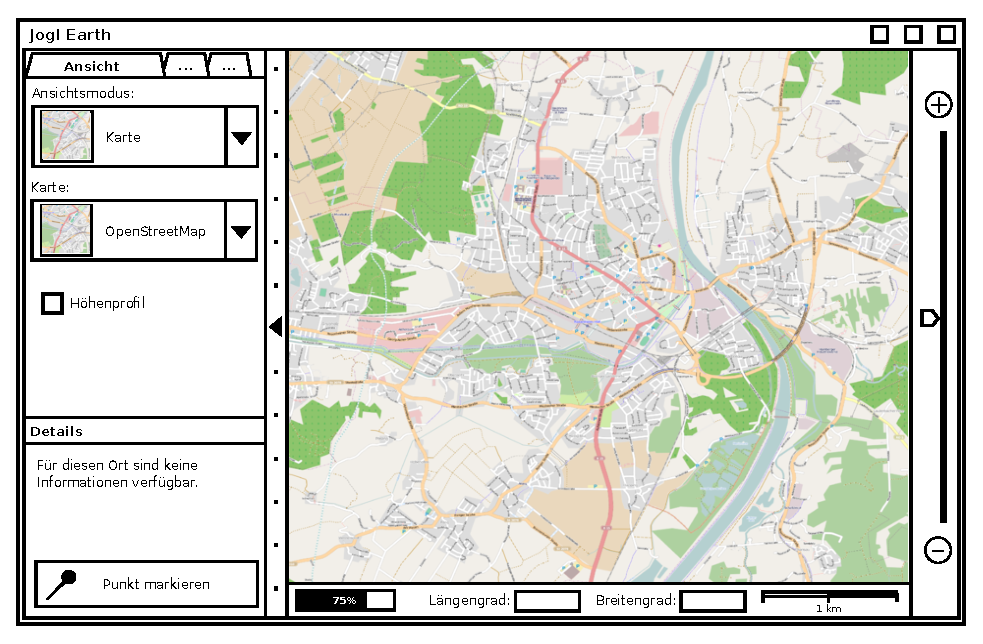
\includegraphics[scale=0.9]{GUI-Ansicht-Strassenkarte.eps}
	\caption{Die Benutzeroberfläche mit gewählter Straßenkarte}
\end{figure}

\begin{figure}
	\centering
		\begin{minipage}[c]{6cm}
        \centering
                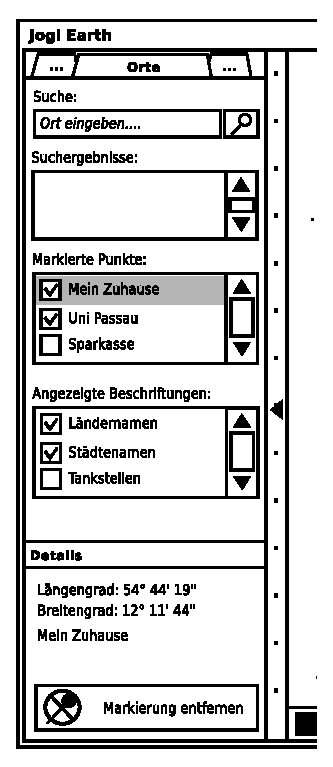
\includegraphics[scale=0.9]{GUI-Orte.eps}
        \end{minipage}
        \begin{minipage}[c]{6cm}
        \centering
                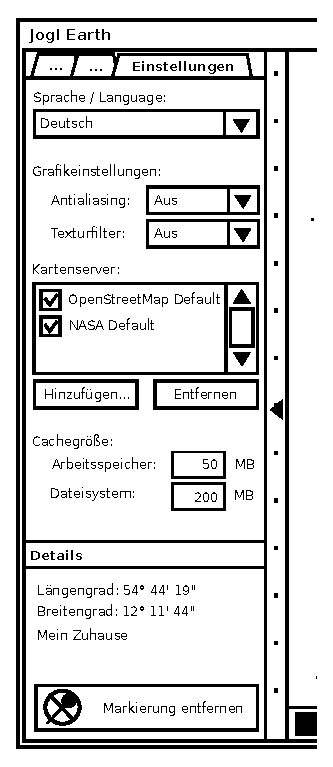
\includegraphics[scale=0.9]{GUI-Einstellungen.eps}
        \end{minipage}
        \caption{Der Orte- und der Einstellungstab}
\end{figure}
\begin{figure}
	\centering
	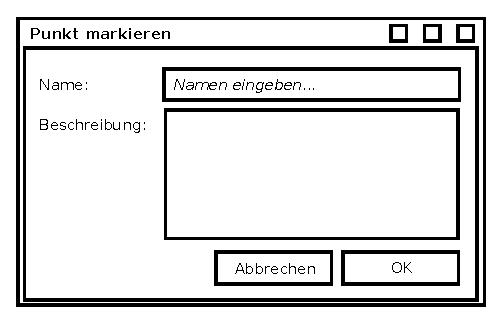
\includegraphics[scale=0.9]{GUI-Markieren.eps}
	\caption{Das Dialogfenster zum Anlegen einer neuen Markierung}
\end{figure}


\begin{figure}
	\centering
	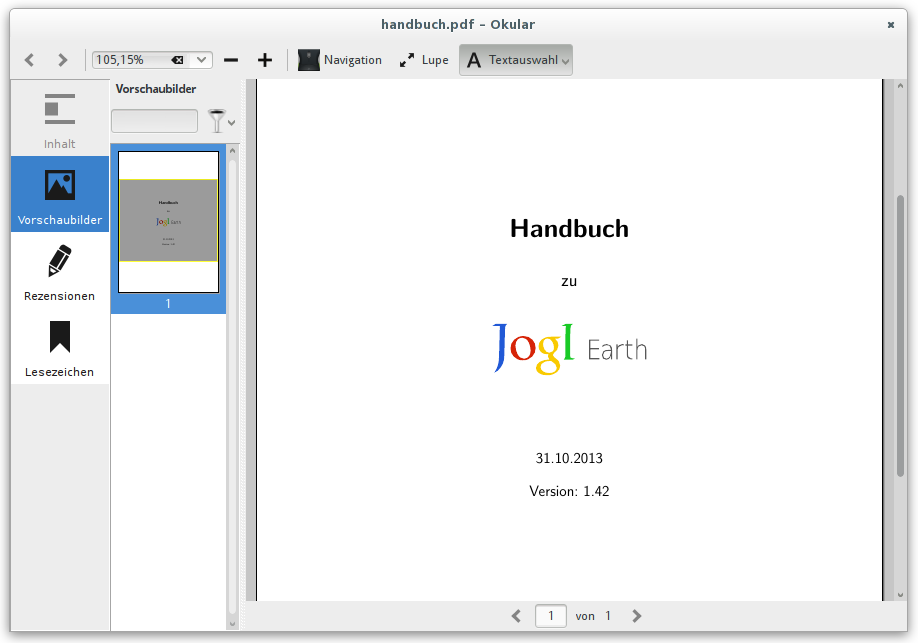
\includegraphics[scale=0.5]{GUI-Handbuch.png}
	\caption{Das Handbuch in einem handelsüblichen PDF-Betrachter}
\end{figure}
\begin{figure}
	\centering
	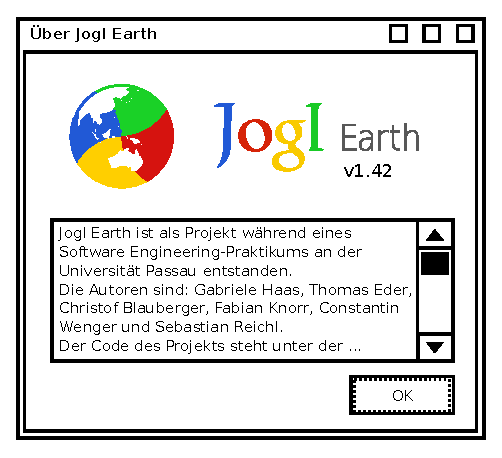
\includegraphics[scale=0.9]{GUI-About.eps}
	\caption{Das Informationsfenster}
\end{figure}

\clearpage
\pagebreak

\section{Steuerung der Kartenansicht}

\vspace{3mm}
\subsection*{Mausbelegung}
\begin{tabular}{|>{\centering \arraybackslash}m{3cm}|m{9cm}|}
\hline

\includegraphics[scale=1.0]{KeyImages/mouseDrag_left.eps} & Drehen der Erdkugel / Verschieben der Karte \\ 
\hline 

\includegraphics[scale=1.0]{KeyImages/mouseDoubleClick_left.eps} & Punkt unter dem Mauszeiger im Kartenfenster zentrieren \\
\hline

\includegraphics[scale=1.0]{KeyImages/mouseDrag_right.eps} & Kippen der Kamera \\
\hline

\includegraphics[scale=1.0]{KeyImages/mouse_scrollen.eps} & Zoomen der Ansicht \\
\hline
\end{tabular} 



\vspace{5mm}
\subsection*{Tastaturbelegung}
\begin{tabular}{|>{\centering \arraybackslash}m{3cm}|m{9cm}|}
\hline
\rule[-1ex]{0pt}{7ex}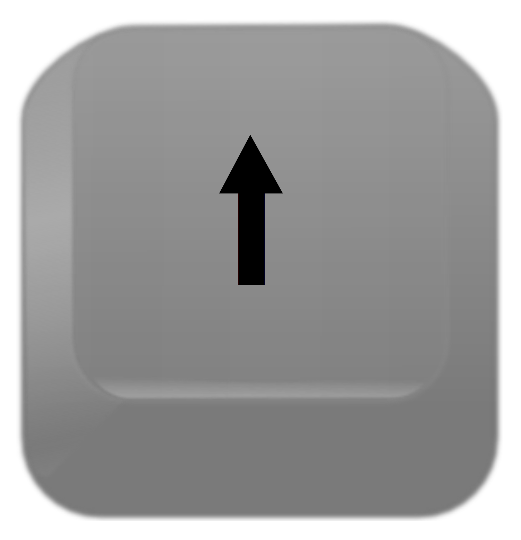
\includegraphics[scale=0.08]{KeyImages/key_arrow_up.eps}& \multirow{3}{*}{Drehen der Erdkugel / Verschieben der Karte}\\
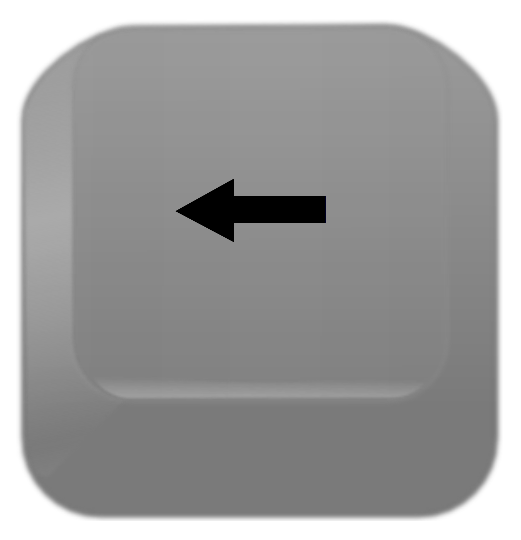
\includegraphics[scale=0.08] {KeyImages/key_arrow_left.eps} 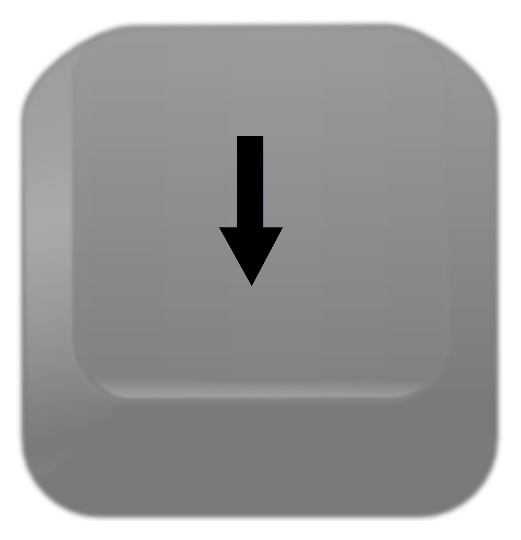
\includegraphics[scale=0.08]{KeyImages/key_arrow_down.eps} 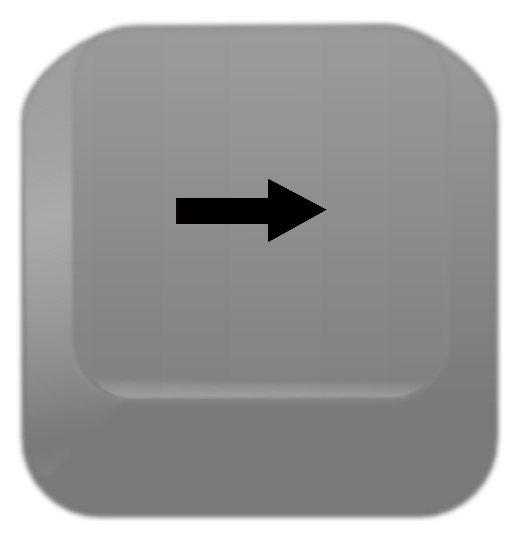
\includegraphics[scale=0.08]{KeyImages/key_arrow_right.eps} &  \\
\hline
\rule[-1ex]{0pt}{7ex} 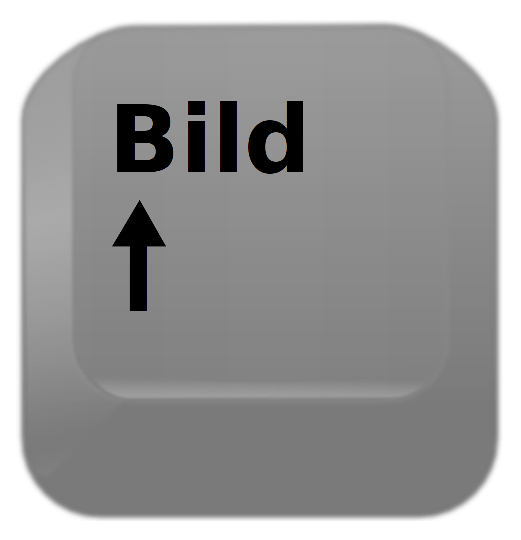
\includegraphics[scale=0.08]{KeyImages/key_Bild_Auf.eps}  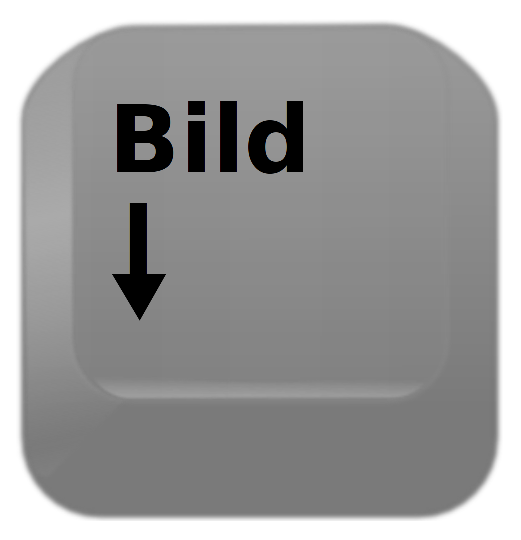
\includegraphics[scale=0.08]{KeyImages/key_Bild_Ab.eps} & Kippen der Kamera nach oben / unten\\
\hline
\rule[-1ex]{0pt}{7ex} 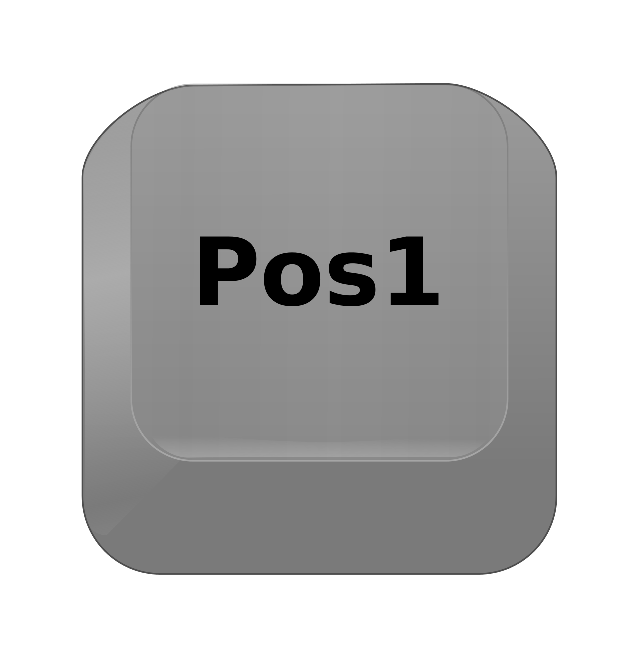
\includegraphics[scale=0.08]{KeyImages/key_Pos1.eps}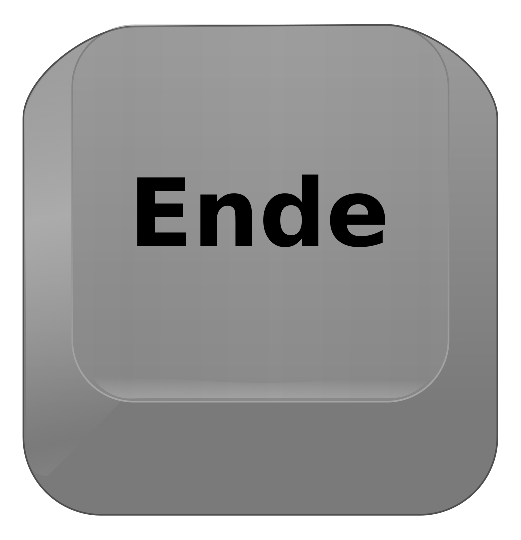
\includegraphics[scale=0.08]{KeyImages/key_Ende.eps} & Kippen der Kamera nach links / rechts \\
\hline
\rule[-1ex]{0pt}{7ex} 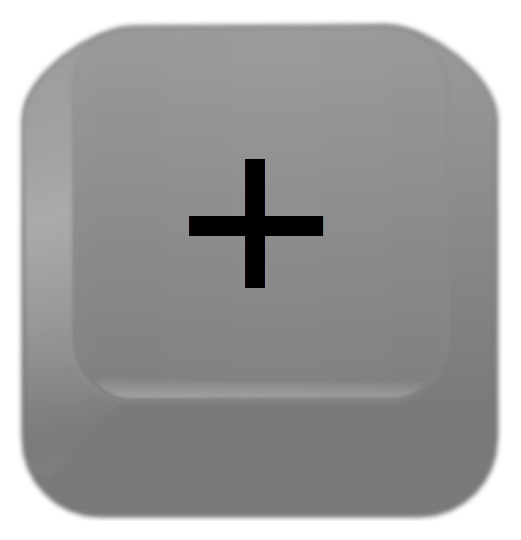
\includegraphics[scale=0.08]{KeyImages/key_Plus.eps}  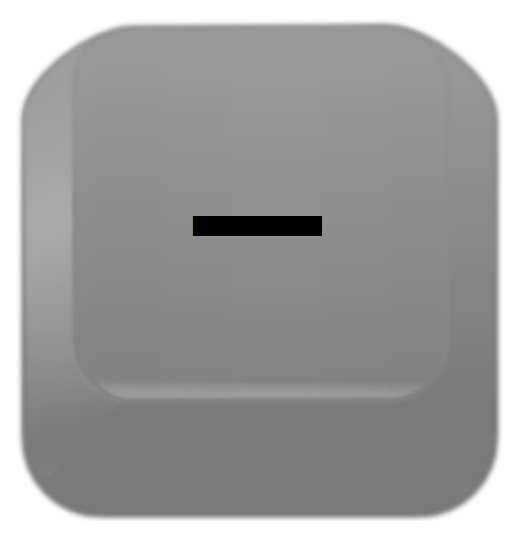
\includegraphics[scale=0.08]{KeyImages/key_Minus.eps} & Zoomen der Ansicht \\
\hline
\rule[-1ex]{0pt}{7ex} 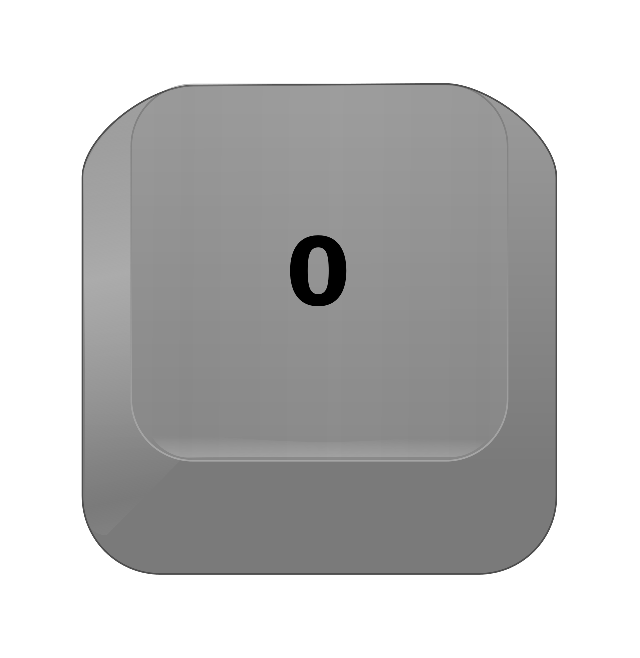
\includegraphics[scale=0.08]{KeyImages/key_0.eps} & Rücksetzen des Kippens \\ 
\hline
\rule[-1ex]{0pt}{7ex} 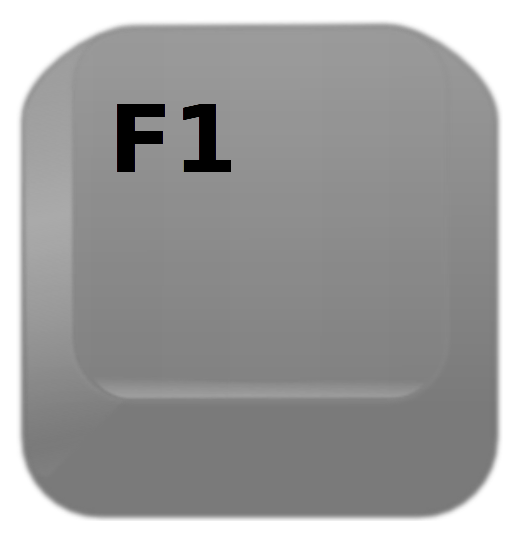
\includegraphics[scale=0.08]{KeyImages/key_F1.eps} & Anzeige des Benutzerhandbuchs \\ 
\hline
\rule[-1ex]{0pt}{7ex} 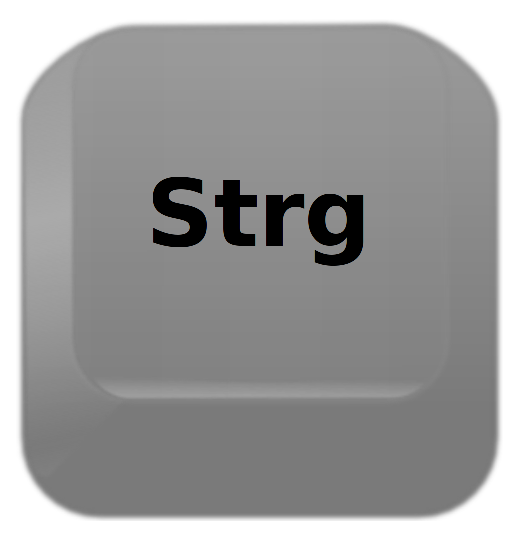
\includegraphics[scale=0.08]{KeyImages/key_Strg.eps} \rule[-1ex]{0pt}{7ex}\raisebox{0.7em}{\textbf{+}} 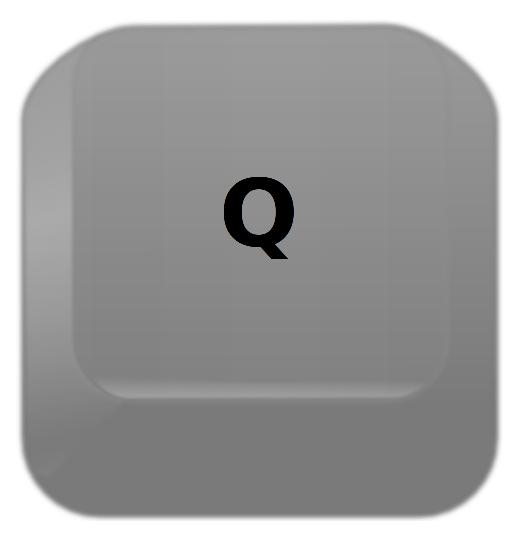
\includegraphics[scale=0.08]{KeyImages/key_Q.eps} & Beenden der Anwendung \\ 
\hline
\end{tabular} 



\chapter{Systemarchitektur}
Die Systemarchitektur folgt dem Model-View-Controller-Pattern.
\vspace{3mm}
\begin{figure}[h]
\centering
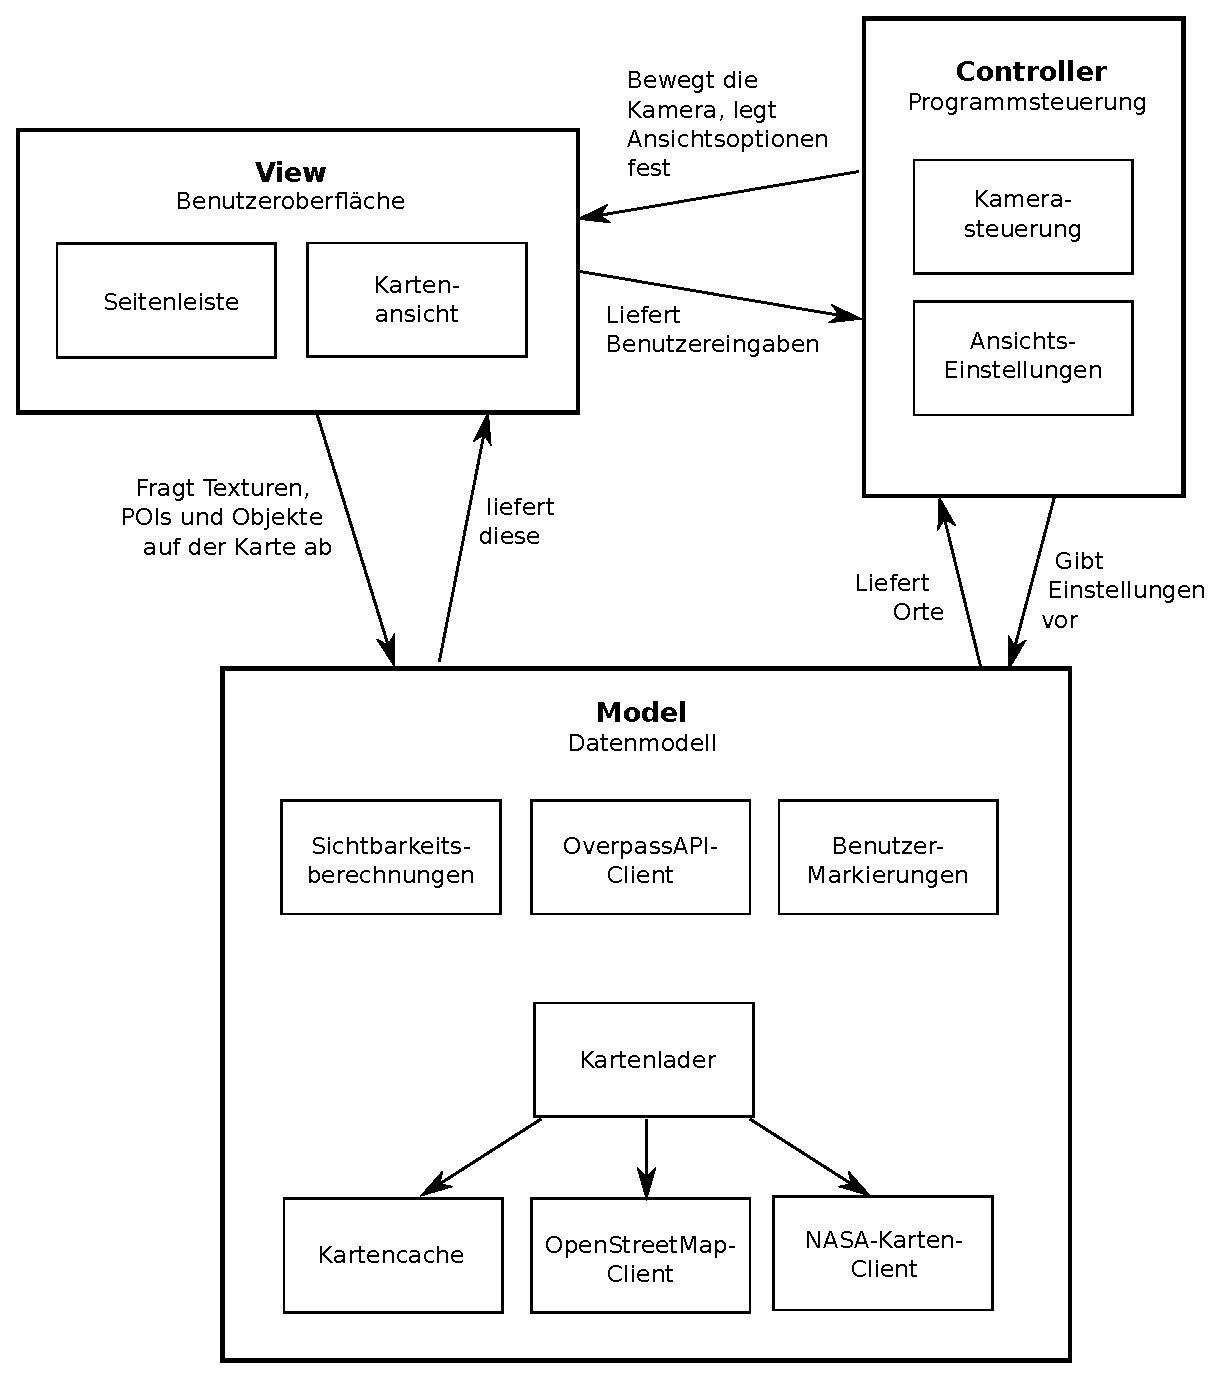
\includegraphics[scale=0.6]{ModelViewController.eps}
\caption{Konzept der Systemarchitektur (Abriss)}
\end{figure}
\subsubsection*{Controller}
Die \textbf{Programmsteuerung} übernimmt die Verarbeitung der Ein- und Ausgaben und steuert die Ansicht.
 Sie ist für die Umsetzung der Nutzerbefehle und gespeicherter Einstellungen verantwortlich.
\subsubsection*{View}
Die \textbf{Benutzeroberfläche} dient als Schnittstelle zwischen Anwender und Programm. Sie erzeugt eine visuelle Darstellung aus den Befehlen der Programmsteuerung und den Daten des Modells. Eingaben wie Tastendrücke oder das Anwählen eines GUI-Elements leitet sie an die Steuerung weiter.

\subsubsection*{Model}
Das \textbf{Datenmodell} ist dafür zuständig, Berechnungen und Anfragen bezüglich der Karte oder des Globus zu beantworten. Es bestimmt die Sichtbarkeit von Kartenabschnitten und beschafft Karten-, Markierungs- sowie ortsspezifische Daten.


\chapter{Produktfunktionen}

\nplpadding{2}
\muss
\renewcommand{\ziellabel}{F}

Wunschkriterien werden mit {\W } gekennzeichnet, alle verbleibenden sind Musskriterien.

\section{Benutzeroberfläche}
\begin{enumerate}[leftmargin=2.2cm]
\item Ändern der Programmfenstergröße 
\item Schließen des Fensters und damit beenden des Programms
\item Ein- und Ausklappen der Seitenleiste
\item Sprachwechsel ohne Neustart
\item Anzeige des Zoomlevels
\item Ändern des Zoomlevels
\item Aktualisieren der Fortschrittsanzeige für im Hintergrund geladene Daten
\item Anzeige des Längen- und Breitengrades des zentrieren Punktes
\item Änderung des aktuellen Längen- und Breitengrades
\item Anzeige des Benutzerhandbuchs
\item Anzeige eines Infofensters (\textit{„About Box“})
\wunsch
\item Anzeige verfügbarer Markierungen
\item Aktivieren und Deaktivieren einer Markierung
\muss
\item Anzeige verfügbarer Overlays
\item Aktivieren und Deaktivieren eines Overlays
\wunsch
\item Suche nach einem Ort im sichtbaren Kartenbereich
\item Globale Suche nach einem Ort
\item Anzeige von Suchergebnissen
\end{enumerate}

\section{Räumliche Berechnungen}
\begin{enumerate}[leftmargin=2.2cm,resume]
\item Erzeugung einer ebenen Globusoberfläche
\item Erzeugung einer flachen Kartenebene
\wunsch
\item Erzeugung einer Globusoberfläche aus einer Heightmap
\item Erzeugung einer Kartenoberfläche aus einer Heightmap
\muss
\item Berechnung des Längen- und Breitengrades unter einem Bildschirmpunkt
\item Berechnung der Bildschirmposition eines Punktes der Karte oder des Globus anhand seiner Koordinaten
\wunsch
\item Berechnung des Maßstabs des Punktes unter dem Anzeigemittelpunkt
\muss
\item Bestimmung der nötigen Kachelauflösung aus der Kameraposition
\item Entscheidung der Sichtbarkeit von Kacheln auf Karte oder Globus aus Kameraposition und Sichtfeld (FOV)
\item Berechnung der Kameraposition und -orientierung aus Mausbewegungen
\item Berechnung der Kameraposition und -orientierung aus Tastatureingaben
\end{enumerate}

\section{Ansichtsfenster}
\begin{enumerate}[leftmargin=2.2cm,resume]
\item Ändern des Ansichtsmodus
\item Ändern des Kartentyps
\wunsch
\item Zu- oder Abschalten des Höhenprofils
\item Ändern des Detaillevels (LOD) des 3D-Modells
\item Ändern der Antialiasing-Einstellung
\item Ändern des Texturfilters
\muss
\item Anzeige von Overlays als zweidimensionale Objekte
\wunsch
\item Anzeige von bestehenden Markierungen
\muss
\item Darstellung des Sternenhimmels als Hintergrund
\item Zentrieren eines Punktes im Ansichtsfenster, der als Längen- und Breitengrad gegeben ist
\item Rendern des 3D-Modells im Ansichtsfenster
\end{enumerate}

\subsection*{Kartenansicht}
\begin{enumerate}[leftmargin=2.2cm,resume]
\item Verschieben der Karte auf der Ebene
\item Kippen der Kamera relativ zu ihrer Position mit der Einschränkung, dass der Bildmittelpunkt immer auf die Karte zeigen muss
\item Verschieben der Kamera senkrecht zur Kartenebene (Zoomen) mit einer oberen und unteren Grenze
\end{enumerate}

\subsection*{Globusansicht}
\begin{enumerate}[leftmargin=2.2cm,resume]
\item Drehen der Erde um ihre Achse
\item Drehen der Erde in Richtung der Pole, aber nicht über sie hinaus
\item Kippen der Kamera relativ zu ihrer Position mit der Einschränkung, dass der Bildmittelpunkt immer auf den Globus zeigen muss
\item Verschieben der Kamera senkrecht zur Globusoberfläche (Zoomen) mit einer oberen und unteren Grenze
\end{enumerate}

\section{Ortsfunktionen}
\begin{enumerate}[leftmargin=2.2cm,resume]
\item Auswahl einer begrenzten Teilmenge aus der Menge aller anzuzeigender Overlays
\wunsch
\item Markieren eines Punktes mit Name und Notiz
\item Entfernen eines markierten Punkts
\muss
\end{enumerate}

\section{Verarbeitung externer Daten}
\begin{enumerate}[resume,leftmargin=2.2cm]
\item Hinzufügen eines Datums zu einem Cache
\item Entfernen eines Datums aus einem vollen Cache mittels einer Verdrängungsstrategie
\item Leeren eines Caches
\item Ändern der maximalen Größe eines Caches
\item Laden einer Textur
\wunsch
\item Laden von SRTM-Höhenprofildaten
\item Auffinden von Informationen über einen Punkt anhand seiner Koordinaten
\muss
\item Auffinden von POIs und Städtenamen in einem Kartenausschnitt via Overpass-API
\wunsch
\item Auffinden von Orten über ihren Namen via Nominatim
\muss
\item Speichern von Einstellungen und Markierungen (\W) in eine Datei
\item Laden von Einstellungen und Markierungen (\W) aus einer Datei
\item Asynchrones Ausführen der Datenoperationen \ziel{F550} - \ziel{F590W}
\end{enumerate}


\chapter{Produktdaten}

\renewcommand{\ziellabel}{D}
\muss

Wunschkriterien werden mit {\W } gekennzeichnet, alle verbleibenden sind Musskriterien.\\

\begin{enumerate}[leftmargin=2cm]
\item Vom Programm angelegte Dateien werden im \textit{Datenverzeichnis}, einem Unterordner des Benutzerverzeichnisses, gespeichert. Unter Windows ist das \texttt{\%LOCALAPPDATA\%}, auf allen anderen Systemen \texttt{\textasciitilde/.joglearth/}
\item Es werden alle benötigten Bibliotheken mitgeliefert, diese sind im einzelnen: 
\begin{itemize}
\item JOGL mit allen betriebssystemabhängigen Bibliotheken
\item die Forms-Bibliothek von JGoodies
\end{itemize}
\item Einstellungen werden in der Datei \texttt{settings.xml} im Datenverzeichnis gespeichert. Zu den darin gespeicherten Daten gehören:
\begin{itemize}
\item die gewählte Sprache
\item die Antialiasing-Einstellung (\W)
\item der gewählte Texturfilter (\W)
\item das eingestellte Detaillevel (\W)
\item ob das Höhenprofil aktiviert wurde (\W)
\item eingestellte Puffergrößen
\item markierte Punkte mit Name und Notiz (\W)
\end{itemize}
\item Zwischengespeicherte Textur- und SRTM-(\W) Kacheln werden im Unterordner \texttt{cache} des Datenverzeichnisses abgelegt. Dabei erhält jede Kombination aus Server- und Kartentyp einen eigenen Unterordner
\item Mitgelieferte Daten, wie beispielsweise die Kinder-Weltkarte, sind direkt in der JAR-Datei enthalten und werden daraus gelesen
\vspace{0.5cm}
\begin{figure}[!htb]
	\centering
	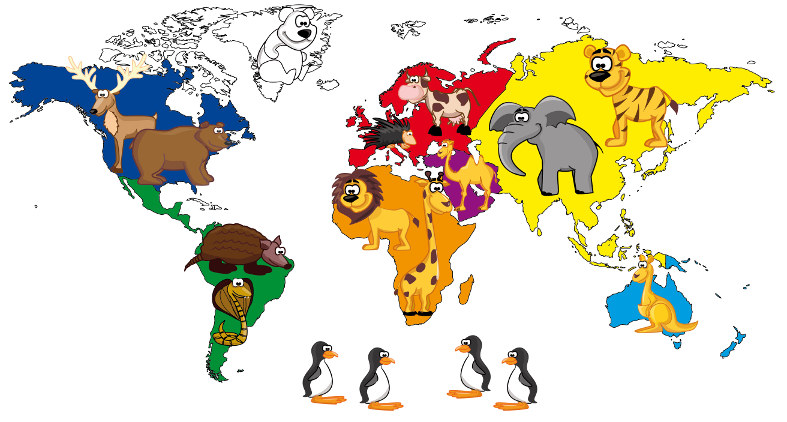
\includegraphics[scale=0.3]{Kinder-Weltkarte.jpg}
\end{figure}
\end{enumerate}


\chapter{Produktleistungen}

\renewcommand{\ziellabel}{L}
\muss

Wunschkriterien werden mit {\W } gekennzeichnet, alle verbleibenden sind Musskriterien.

\begin{enumerate}[leftmargin=2.2cm]
\item Die Benutzeroberfläche ist grafisch ansprechend, gut strukturiert und intuitiv verständlich gehalten
\wunsch
\item Um auch Kinder zu motivieren, \JoglEarth zu verwenden, wird eine altersgemäße Kinder-Weltkarte angeboten
\muss
\item Die Oberfläche wird in den Sprachen Englisch und Deutsch angeboten.
\item Die gesamte GUI ist komfortabel mit Maus und Tastatur steuerbar
\item Die einklappbare Seitenleiste bietet dem Benutzer die Möglichkeit, einen größeren Umfang des Kartenmaterials zu sehen
\item Es treten keine Darstellungsfehler (wie Durchdringen der Kartenebene) durch ungünstige Kamerapositionen und -einstellungen auf
\item Es wird versucht, die Lesbarkeit von Beschriftungen auch bei einer hohen Zahl von Overlays akzeptabel zu halten
\item Der Nutzer findet durch die Markierungsfunktion für ihn interessante Punkte wieder
\item Eine sprachunabhängige Suchfunktion unterstützt den Nutzer, POIs oder Orte unkompliziert aufzufinden
\item Unnötiges Nachladen und Speicherverbrauch werden minimiert, indem Karten- und Höhendaten werden effizient zwischengespeichert werden.
\item Durch Sichtbarkeitsberechnungen und intelligentes Vorausladen wird gleichzeitig die Wartezeit und die Menge unnötig geladener Daten gering gehalten
\item Hintergrundvorgänge des Programms wie das Nachladen von Kartendaten unterbrechen den Rendervorgang nicht
\item Ist eine Textur nicht verfügbar oder wird sie geladen, ist dies an einer Platzhaltertextur in der Ansicht erkennbar
\wunsch
\item Der Energieverbrauch wird minimiert, indem Rendervorgänge nur bei Bildänderungen gestartet werden
\item Die Anwendung ist intuitiv mit der Toucheingabe auf Windows 8 bedienbar
\item Durch anpassbare Grafikeinstellungen bleibt die Leistung auch auf älterer Hardware akzeptabel
\item Mit zusätzlichen Darstellungsmöglichkeiten wie Höhenprofilen, einer Sonnensystem-\\Modellansicht und einem Sternenhimmel als Hintergrundmotiv werden die Ansichten optisch aufgewertet
\end{enumerate}



\chapter{Qualitätsbestimmungen}


\vspace{1cm}
\begin{center}
\begin{tabular}{lcccc}
\hline 
\rule[-1ex]{0pt}{4ex} \textit{Produktqualität} & \textit{sehr gut} & \textit{gut} & \textit{normal} & \textit{nicht relevant} \\ 
\hline 
\rule[-1ex]{0pt}{4ex} \textbf{Funktionalität} &  &  &  &  \\ 
\rule[-1ex]{0pt}{4ex} \hspace{10pt} Web-Mining & &  & • & \\ 
\rule[-1ex]{0pt}{4ex} \hspace{10pt} Interoperabilität & & • & & \\ 

\hline 
\rule[-1ex]{0pt}{4ex} \textbf{Zuverlässigkeit} &  &  &  &  \\ 
\rule[-1ex]{0pt}{4ex} \hspace{10pt} Stabilität & • & & & \\ 
\rule[-1ex]{0pt}{4ex} \hspace{10pt} Fehlertoleranz & • & & & \\ 
\rule[-1ex]{0pt}{4ex} \hspace{10pt} Wiederherstellbarkeit &  &  &  & • \\ 

\hline 
\rule[-1ex]{0pt}{4ex} \textbf{Benutzbarkeit} &  &  &  &  \\ 
\rule[-1ex]{0pt}{4ex} \hspace{10pt} Bedienbarkeit & • & & & \\ 
\rule[-1ex]{0pt}{4ex} \hspace{10pt} Erlernbarkeit & • & & & \\ 
\rule[-1ex]{0pt}{4ex} \hspace{10pt} Grafische Gestaltung & & • & & \\ 
\rule[-1ex]{0pt}{4ex} \hspace{10pt} Verständlichkeit & • & & & \\ 

\hline 
\rule[-1ex]{0pt}{4ex} \textbf{Effizienz} &  &  &  &  \\ 
\rule[-1ex]{0pt}{4ex} \hspace{10pt} Bildqualität & & • & & \\ 
\rule[-1ex]{0pt}{4ex} \hspace{10pt} Laufzeit & & • & & \\ 
\rule[-1ex]{0pt}{4ex} \hspace{10pt} Speichermanagement & • & & & \\ 

\hline 
\rule[-1ex]{0pt}{4ex} \textbf{Anpassungsfähigkeit} &  &  &  &  \\ 
\rule[-1ex]{0pt}{4ex} \hspace{10pt} Code-Qualität & & • & & \\ 
\rule[-1ex]{0pt}{4ex} \hspace{10pt} Modifizierbarkeit & & & • & \\ 

\hline 
\rule[-1ex]{0pt}{4ex} \textbf{Portierbarkeit} &  &  &  &  \\ 
\rule[-1ex]{0pt}{4ex} \hspace{10pt} Erweiterbarkeit & & & • & \\ 
\rule[-1ex]{0pt}{4ex} \hspace{10pt} Konformität & & • & & \\ 

\hline 
\rule[-1ex]{0pt}{4ex} \textbf{Dokumentation} & • & & & \\ 
\hline 
\end{tabular} 
\end{center}

\pagebreak



\section*{Funktionalität}
\begin{details}
\item \sfbf{Web Mining:} Die Automatische Extraktion von Informationen aus dem Internet. Bei \JoglEarth findet das Web Mining bei der Suchfunktion Anwendung. Um die Benutzeroberfläche übersichtlich zu halten, ist nur eine einfache Suche nach Wortteilen möglich, die nicht weiter eingegrenzt wird. 

\item \textbf{Interoperabilität:} Die Anwendung soll mit OpenStreetMap, der Overpass-API und ähnlichen Diensten interagieren um das Kartenmaterial mit Zusatzinformationen grafisch zu unterstützen. Da dies Kernbestandteil ist, wird darauf besonders Wert gelegt.
\end{details}


\section*{Zuverlässigkeit}
\begin{details}
\item \sfbf{Stabilität:} Die Lauffähigkeit des Programms soll nicht unterbrochen oder beeinträchtigt werden. Programmabstürze und Fehlverhalten führen sehr schnell zur Unzufriedenheit beim Benutzer, weswegen der Stabilität hohe Priorität zukommt.

\item \sfbf{Fehlertoleranz:} Das Programm soll trotz fehlerhafter Eingaben seitens des Anwenders seine Funktionsweise aufrechterhalten. Dies ist ein wichtiger Punkt, da falsche Behandlung von unsinnigen Eingaben zu Fehlverhalten führt (\textref{Stabilität}).

\item \sfbf{Wiederherstellbarkeit:} Bei Neustart nach unsachgemäßer Beendigung des Programms, z.B. durch einen Systemabsturz, verhält sich das Programm wie bei einem normalen Start. In der \texttt{settings}-Datei gespeicherte Einstellungen werden angewendet; Änderungen, die in der abgestürzten Sitzung vorgenommen wurden, können unter Umständen verloren gehen. Es wird kein Versuch unternommen, die letzte Sitzung wiederherzustellen, da der Zustand keine wirklich kritischen Informationen enthält.
\end{details}


\section*{Benutzbarkeit}
\begin{details}
\item \sfbf{Bedienbarkeit:} Die Oberfläche soll intuitiv bedienbar sein. Dies ist auch deshalb von Bedeutung, da Kinder zur Zielgruppe gehören.

\item \sfbf{Erlernbarkeit:} Die Bedienung der Oberfläche soll einfach verstanden werden. Dies deckt sich mit der Anforderung nach intuitiver Bedienbarkeit.

\item \sfbf{Grafische Gestaltung:} Die Oberfläche soll optisch ansprechend wirken. Dabei wird auch auf Einfachheit geachtet, was wiederum der Erlernbarkeit dient.

\item \sfbf{Verständlichkeit:} Die Oberfläche soll selbsterklärend sein. Dieses Ziel ist leicht erreichbar, da der Funktionsumfang gut strukturiert ist.
\end{details}


\section*{Effizienz}
\begin{details}
\item \sfbf{Bildqualität:} Die Satellitenbilder und Kartendaten sollen in bestmöglicher Qualität dargestellt werden, außerdem sollen Bildänderungen flüssig erfolgen. Dies ist für die Sichtbarkeit von Kartendetails und für die Bedienbarkeit unabdinglich.

\item \sfbf{Laufzeit:} Trotz bestmöglicher Bildqualität sollen die Wartezeiten zum Laden der Daten gering gehalten werden. Die Zielsetzung ist es, dabei heutige Standards der Antwortzeit zu erreichen.

\item \sfbf{Speichermanagement:} Die Kacheldaten werden im Dateisystem und im Arbeitsspeicher effizient gepuffert. Eine gute Umsetzung dieses Punktes wirkt sich unmittelbar auf die Ladezeiten aus, weswegen es höchste Aufmerksamkeit genießt.
\end{details}


\section*{Anpassungsfähigkeit}
\begin{details}
\item \sfbf{Code-Qualität:} Der Quellcode des Programms soll verständlich gehalten werden. Dies ist für die Teamarbeit unerlässlich.

\item \sfbf{Modifizierbarkeit:} Zusätzliche Änderungen bzw. Anpassungen des Codes sollen einfach umsetzbar sein. Da die Software nach Beendigung des Projekts nicht weiterentwickelt wird, spielt dies eine untergeordnete Rolle.
\end{details}


\section*{Portierbarkeit}
\begin{details}
\item \sfbf{Erweiterbarkeit:} Zusätzliche Funktionalitäten sollen in den Code integrierbar sein. Hier gilt das selbe wie für die Modifizierbarkeit.

\item \sfbf{Konformität:} Im Software Engineering etablierte Konventionen zum Codedesign sollen eingehalten werden.
\end{details}


\section*{Dokumentation}
\begin{details}
\item \sfbf{Dokumentation:} Ein gutes Softwareprodukt zeichnet sich unter Anderem durch die Qualität des Benutzerhandbuchs, der Quelltextdokumentation und der einzelnen Phasendokumente aus. Sie sollen gut strukturiert, leicht verständlich und fachlich kompetent gehalten sein. 
\end{details}




\chapter{Globale Testszenarien und Testfälle}

\renewcommand{\ziellabel}{T}

\begin{details}[2pt]
\item \sfbf{Ausgangspunkt:} Nackte Grundinstallation 
\item \sfbf{Voraussetzung:} keine
\item \sfbf{Testszenario:} Anwendungsstart
\end{details}
\vspace{2mm}
\begin{enumerate}[leftmargin = 2.2cm]
\item Starten des Programms.\\Es öffnet sich das Hauptfenster in der Systemsprache oder (ersatzweise) Englisch (\ziel{F040}). Der Ansichts-Tab befindet sich im Vordergrund.
\wunsch
\item Die GUI startet im Sonnensystemmodus. Die Auswahl des Kartentyps und des Höhenprofils, die Anzeigen für Längen-, Breitengrad, Maßstab (\W) und Zoomlevel entfällt (gemäß Abbildung 5.1).
\muss
\item Der Hintergrund zeigt einen Sternenhimmel (\ziel{F380}).
\item Sollte der Sonnensystemmodus (\W) nicht realisiert werden, startet die GUI in der Globus-Ansicht mit Satellitenbildern. (\ziel{F300}).
\item Klick auf den Rand der Seitenleiste (vgl. Abbildung 5.1).\\ Die Seitenleiste wird ausgeblendet; der Rand ist zum wiedereinblenden anklickbar (\ziel{F030})\\Klick auf den Rand der Seitenleiste.\\Die Seitenleiste wird wieder eingeblendet (\ziel{F030}).
\item Klick auf den Einstellungen-Tab.\\Klick auf die Handbuchschaltfläche.\\Das Handbuch öffnet sich in einem neuen Fenster (\ziel{F100}).\\Schließen des Handbuchfensters.\\ Das Handbuchfenster schließt sich.
\item Klick auf die Infoschaltfläche.\\Das Infofenster öffnet sich (\ziel{F110}).\\Schließen des Infofensters.
\item Ändern der Sprache.\\Die Anzeigesprache ändert sich.\\ Rücksetzen der Sprache (\ziel{F040}).\\Die Anzeigesprache ändert sich erneut.
\end{enumerate}

\newpage
\vspace{1.0cm}
\begin{details}[2pt]
\item \sfbf{Ausgangspunkt:} Nackte Grundinstallation 
\item \sfbf{Voraussetzung:} Szenario Anwendungsstart
\item \sfbf{Testszenario:} Globusansicht
\end{details}
\vspace{2mm}
\begin{enumerate}[leftmargin = 2.2cm, resume]
\item Wechsel zum Ansicht-Tab.\\
Auswahl der Globusansicht, falls der Sonnensystemmodus (\W) aktiv ist.\\Der Ansichtsmodus ändert sich entsprechend (\W).\\
Es ist die Erdkugel mit Satellitenbildern sichtbar (\ziel{F190}, \ziel{F300}).
\item Ändern des Kartentyps zu OpenStreetMap-Straßenkarten.\\Der Kartentyp ändert sich ensprechend (\ziel{F310}).
\item Das Zoomlevel ist auf der niedrigsten Einstellung (\ziel{F050})
\item Momentanen Maßstab und Koordinaten (Längen-/Breitengrad) notieren (\ziel{F080}, \ziel{F250W}).\\Ändern des Zoomlevels auf 50\% (\ziel{F060}).\item Der Maßstab ändert sich entsprechend (\ziel{F250W}).
\item Die Koordinaten des Mittelpunkts (der angezeigte Längen- und Breitengrad) bleibt gleich (\ziel{F080}, \ziel{F230}, \ziel{F460}).
\item Die Globusoberfläche zeigt eine Platzhaltertextur, die Stück für Stück durch nachgeladene Kartenkacheln ersetzt wird (\ziel{F260}, \ziel{F270}, \ziel{F540}).
\item Der Ladefortschritt wird in der Statusleiste angezeigt (\ziel{F070}). \item Die Oberfläche bleibt während des Ladevorgangs bedienbar (\ziel{F610}).
\item Zoomlevel wieder rücksetzen auf das Minimum (\ziel{F060}).\\ Maßstabsanzeige vergleichen mit vorheriger Skalierung ( \ziel{F250W}).
\end{enumerate}


\vspace{1.0cm}
\begin{details}[2pt]
\item \sfbf{Ausgangspunkt:} Nackte Grundinstallation 
\item \sfbf{Voraussetzung:} Szenario Globusansicht
\item \sfbf{Testszenario:} Navigation auf dem Globus
\end{details}
\vspace{2mm}
\begin{enumerate}[leftmargin = 2.2cm, resume]
\item Im Ansichtsfenster die Maus mit gedrückter linker Taste nach links und rechts verschieben.\\Der Globus dreht sich um die Erdachse in Bewegungsrichtung der Maus (\ziel{F280}, \ziel{F430}).
\item Im Ansichtsfenster die Maus mit gedrückter linker Taste nach oben und unten verschieben.\\Der Globus dreht sich in Bewegungsrichtung der Maus in Richtung Nord- oder Südpol, aber nicht über die Pole hinaus (\ziel{F440})
\item Im Ansichtsfenster die Maus mit gedrückter linker Taste nach links und rechts verschieben.\\Der Globus dreht sich weiterhin um die Erd- und nicht um eine andere Achse (\ziel{F280}, \ziel{F430}).
\item Hineinzoomen auf 80-90\%.\\ Das Zoomlevel ändert sich entsprechend (\ziel{F060}).\\ Warten, bis die Kartenkacheln geladen sind.
\wunsch
\item Aktivieren des Höhenprofils. (\ziel{F320W}).\\ Nach einer eventuellen Ladezeit wird die Globusoberfläche den SRTM-Höhendaten entsprechend nach oben oder unten versetzt angezeigt (\ziel{F210W}, \ziel{F550W}).
\muss
\item Im Ansichtsfenster die Maus mit gedrückter rechter Taste nach oben, unten, links und rechts bewegen.\\Die Ansicht wird am Kameraursprung entsprechend der Bewegungen gekippt (\ziel{F450})
\wunsch
\item Das Höhenprofil ist von der Seite betrachtbar.\\Wechsel zum Einstellungen-Tab.\\Verändern der Antialiasing-Einstellung (\ziel{F340W}).\\Ist Antialiasing auf dem System verfügbar, werden Objektkanten bei Aktivierung geglättet.
\item Ändern der Texturfilter-Einstellungen (\ziel{F350W}).\\Ist ein Texturfilter (z.B. anisotrope Filterung) auf dem System verfügbar, erscheinen perspektivisch verzerrte Oberflächen schärfer.
\muss
\item Die Ansicht ist gekippt.\\Im Ansichtsfenster die Maus mit gedrückter linker Taste in alle Richtungen verschieben.\\Der Globus dreht sich, konsistent mit vorherigen Drehungen, unter dem Betrachter durch (\ziel{F280}, \ziel{F430}).
\item Rücksetzen des Kippens mit der Taste \textit{0} (\ziel{F290}, \ziel{F450})
\item Schließen des Fensters (\ziel{F020}).\\Programm wird beendet.
\end{enumerate}



\vspace{1.0cm}
\begin{details}[2pt]
\item \sfbf{Ausgangspunkt:} Nackte Grundinstallation 
\item \sfbf{Voraussetzung:} Szenario Anwendungsstart
\item \sfbf{Testszenario:} Kartenansicht
\end{details}
\vspace{2mm}
\begin{enumerate}[leftmargin = 2.2cm, resume]
\item Wechsel zum Ansicht-Tab.\\
Auswahl der Kartenansicht.\\Der Ansichtsmodus ändert sich entsprechend.\\
Es ist eine flache Kartenebene mit Satellitenbildern sichtbar (\ziel{F200}, \ziel{F300}).
\item Ändern des Kartentyps zu OpenStreetMap-Straßenkarten.\\Der Kartentyp ändert sich ensprechend (\ziel{F310}).
\item Das Zoomlevel ist auf der niedrigsten Einstellung (\ziel{F050})
\item Momentanen Maßstab und Koordinaten (Längen-/Breitengrad) notieren (\ziel{F080}, \ziel{F250W}).\\Ändern des Zoomlevels auf 50\% (\ziel{F060}).\item Der Maßstab ändert sich entsprechend (\ziel{F250W}).
\item Die Koordinaten des Mittelpunkts (der angezeigte Längen- und Breitengrad) bleibt gleich (\ziel{F080}, \ziel{F230}, \ziel{F420}).
\item Die Kartenebene zeigt eine Platzhaltertextur, die Stück für Stück durch nachgeladene Kartenkacheln ersetzt wird (\ziel{F260}, \ziel{F270}, \ziel{F540}).
\item Der Ladefortschritt wird in der Statusleiste angezeigt (\ziel{F070}). \item Die Oberfläche bleibt während des Ladevorgangs bedienbar (\ziel{F610}).
\item Zoomlevel wieder rücksetzen auf das Minimum (\ziel{F060}).\\ Maßstabsanzeige vergleichen mit vorheriger Skalierung ( \ziel{F250W}).
\end{enumerate}

\newpage
\vspace{1.0cm}
\begin{details}[2pt]
\item \sfbf{Ausgangspunkt:} Nackte Grundinstallation 
\item \sfbf{Voraussetzung:} Szenario Kartenansicht
\item \sfbf{Testszenario:} Navigation auf der Kartenebene
\end{details}
\vspace{2mm}
\begin{enumerate}[leftmargin = 2.2cm, resume]
\item Im Ansichtsfenster abwechselnd die linke, rechte, obere und untere Pfeiltaste drücken.\\Der Karte verschiebt sich in die entsprechenden Richtungen (\ziel{F290}, \ziel{F400}).
\item Hineinzoomen auf 80-90\%.\\ Das Zoomlevel ändert sich entsprechend (\ziel{F060}).\\ Warten, bis die Kartenkacheln geladen sind.
\wunsch
\item Aktivieren des Höhenprofils. (\ziel{F320W}).\\ Nach einer eventuellen Ladezeit wird die Kartenebene den SRTM-Höhendaten entsprechend nach oben oder unten versetzt angezeigt (\ziel{F220W}, \ziel{F550W}).
\muss
\item Im Ansichtsfenster die Tasten Bild Auf, Bild Ab, Pos1 und Ende drücken.\\Die Ansicht wird am Kameraursprung entsprechend der Tastenbelegung in Kapitel 5.2 gekippt (\ziel{F410})
\wunsch
\item Das Höhenprofil ist nun von der Seite betrachtbar.\\Wechsel zum Einstellungen-Tab.\\Änderung des Detaillevels (LOD) (\ziel{F330W}).\\Der Detailgrad der Höhenprofil-Darstellung ändert sich.\\Wechsel zum Ansichts-Tab.
\muss
\item Die Ansicht ist gekippt.\\ Im Ansichtsfenster die Pfeiltasten betätigen.\\Die Kartenebene bewegt sich konsistent mit den vorherigen Bewegungen unter dem Betrachter durch (\ziel{F290}, \ziel{F400}).
\item Rücksetzen des Kippens mit der Taste \textit{0} (\ziel{F290}, \ziel{F420}).
\item Ändern der Fenstergröße (\ziel{F010}).\\GUI Elemente richten sich neu aus. Wenn die Einstellungsleiste stark verkleinert wird, verschwinden die GUI Elemente.
\item Schließen des Fensters (\ziel{F020}).\\Programm wird beendet.
\end{enumerate}


\vspace{1.0cm}
\begin{details}[2pt]
\item \sfbf{Ausgangspunkt:} Nackte Grundinstallation 
\item \sfbf{Voraussetzung:} Szenario Kartenansicht
\item \sfbf{Testszenario:} Overlays
\end{details}
\vspace{2mm}
\begin{enumerate}[leftmargin = 2.2cm, resume]
\item Wechsel zum Orte-Tab.\\Anzeigen verschiedener Overlays (\ziel{F140}).
\item Die entsprechenden Overlays werden eingeblendet (\ziel{F360}).
\item Aktivieren aller Overlays (\ziel{F150}).
\item Prüfen anhand mehrerer Großstädte, die Menge der angezeigten Overlays (\ziel{F570}).\\Ändern des Zoomlevels auf 70-80\% (\ziel{F060}).
\item Die Anzahl der Labels bleibt in einem angemessenen Rahmen, sodass Beschriftungen lesbar bleiben und die Menge der POIs nicht überwältigend wirkt (\ziel{F470}).
\item Doppelklick auf ein beliebiges angezeigtes Symbol.\\Der POI wird im Ansichtsfenster zentriert (\ziel{F240}, \ziel{F390}).
\wunsch
\item Prüfen ob im Detailfenster die Informationen zum zentrierten Punkt erscheinen (\ziel{F560W}).
\muss
\item Deaktivieren aller Overlays, außer Städte- und Ländernamen (\ziel{F150}).
\end{enumerate}


\vspace{1.0cm}
\begin{details}[2pt]
\item \sfbf{Ausgangspunkt:} Nackte Grundinstallation 
\item \sfbf{Voraussetzung:} Szenario Kartenansicht
\item \sfbf{Testszenario:} Lokale Suche
\end{details}
\vspace{2mm}
\begin{enumerate}[leftmargin = 2.2cm, resume]
\item Eingabe des Längengrades: 48 und des Breitengrades: 13 in der Benutzeroberfläche (\ziel{F090}, \ziel{F390}).\\Ändern des Zoomlevels auf 40-50\% (\ziel{F060}).\\Der Kartenausschnitt im Umkreis von \textit{Salzburg - Österreich} erscheint.
\wunsch
\item Wechsel zum Orte-Tab.\\Auswahl der Option \textit{in der Umgebung} suchen.\\Eingabe des Suchbegriffs \textit{Laufen} (\ziel{F160W}).
\item Der Suchbegriff erscheint im Feld der Suchergebnisse (\ziel{F180W}).
\item Klick auf das erste Suchergebnis.\\Zentrieren des Orts im Ansichtsfenster (\ziel{F240}, \ziel{F390}).
\end{enumerate}


\vspace{1.0cm}
\begin{details}[2pt]
\item \sfbf{Ausgangspunkt:} Nackte Grundinstallation 
\item \sfbf{Voraussetzung:} Szenario Globusansicht
\item \sfbf{Testszenario:} Globale Suche
\end{details}
\vspace{2mm}
\begin{enumerate}[leftmargin = 2.2cm, resume]
\wunsch
\item Ändern des Zoomlevels auf 25-40\% (\ziel{F060}).\\Wechsel zum Orte-Tab.\\Auswahl der Suchoption \textit{Global}.\\Eingabe des Suchbegriffs \textit{Passau} (\ziel{F170W}).
\item Der Suchbegriff erscheint im Feld der Suchergebnisse (\ziel{F180W}).
\item Klick auf ein beliebiges Suchergebnis.\\Zentrieren des Orts im Ansichtsfenster (\ziel{F240}, \ziel{F390}).
\item Eingabe des Suchbegriffs \textit{Ingolstadt} (\ziel{F170W}, \ziel{F580W}).
\item Der Suchbegriff erscheint im Feld der Suchergebnisse (\ziel{F180W}).
\end{enumerate}

\newpage
\vspace{1.0cm}
\begin{details}[2pt]
\item \sfbf{Ausgangspunkt:} Nackte Grundinstallation 
\item \sfbf{Voraussetzung:} Szenario Kartenansicht
\item \sfbf{Testszenario:} Punkte markieren
\end{details}
\vspace{2mm}
\begin{enumerate}[leftmargin = 2.2cm, resume]
\wunsch
\item Wiederholung des Testfalls \ziel{T570}.\\Aktivieren der Overlays \textit{Städtenamen} (\ziel{F150}).
\item Doppelklick auf die Stadt Salzburg.\\Zentrieren der Stadt im Ansichtsfenster (\ziel{F240}, \ziel{F390}).\\Klick auf den Button \textit{Punkt markieren}.\\Der Dialog (gemäß Abbildung 5.7) öffnet sich (\ziel{F480W}).\\Eintragen von Name und Notiz zur Stadt.\\Klick auf OK.\\Der Dialog schließt sich.
\item Wechsel zum Orte-Tab.\\Anzeige der gespeicherten Markierungen (\ziel{F120W}).\\Die Markierungen sind standardmäßig aktiviert.\\Kontrolle, ob der markierte Punkt im Kartenausschnitt angezeigt wird (\ziel{F370W}).\\Notieren der Koordinaten des Punkts.
\item Deaktivieren des soeben markierten Punkts (\ziel{F130W}) \\Die Markierung wird ausgeblendet.
\item Markierung eines weiteren Punkts durch Wiederholung von \ziel{T660W} - \ziel{680W} mit anderem Ort.
\item Auswählen einer der soeben gesetzten Markierungen (\ziel{F120W}).
\item Deaktivieren aller Markierungen (\ziel{F130W}).
\item Klick auf den Button \textit{Markierung entfernen}.\\Die Markierung wird aus der Liste gelöscht (\ziel{F490W}).
\item Schließen des Fensters (\ziel{F020}).\\Einstellungen und markierte Punkte werden gespeichert (\ziel{F590}).\\Programm wird beendet.
\end{enumerate}


\vspace{1.0cm}
\begin{details}[2pt]
\item \sfbf{Ausgangspunkt:} Szenario Punkte markieren wurde erfolgreich ausgeführt
\item \sfbf{Voraussetzung:} Szenario Kartenansicht
\item \sfbf{Testszenario:} Kontrolle der Einstellungen nach Neustart
\end{details}
\vspace{2mm}
\begin{enumerate}[leftmargin = 2.2cm, resume]
\item Starten des Programms.\\Es öffnet sich das Hauptfenster in der Systemsprache oder (ersatzweise) Englisch (\ziel{F040}). Der Ansichts-Tab befindet sich im Vordergrund.
\item Laden der Einstellungen (\ziel{F600}).\\Einstellungen werden übernommen.
\item Wechseln in den Orte-Tab.\\Kontrolle ob die gespeicherten, markierten Punkte vorhanden und deaktiviert sind (\ziel{F120W}).
\item Aktivieren eines gespeicherten Punkts (\ziel{F130W}).\\Zentrieren des Punkts im Ansichtsfenster (\ziel{F240}, \ziel{F390}).\\Vergleich der Koordinaten auf Übereinstimmung mit den zuvor Notierten.
\end{enumerate}


\vspace{1.0cm}
\begin{details}[2pt]
\item \sfbf{Ausgangspunkt:} Nackte Grundinstallation 
\item \sfbf{Voraussetzung:} Szenario Anwendungsstart
\item \sfbf{Testszenario:} Caching, Diverses
\end{details}
\vspace{2mm}
\begin{enumerate}[leftmargin = 2.2cm, resume]
\item Eingabe von ungültigen Längen- und/ oder Breitengraden.\\ Ansicht wird nicht geändert.
\item Auswahl des Kartentyps \textit{Kinder-Weltkarte} (\ziel{F310}).\\Der Globus mit der Kinder-Weltkarte wird angezeigt.
\item Auswahl des Kartentyps OpenStreetMap.\\Beobachten der Größe des Ordners \texttt{cache} im Datenverzeichnis mit einem geeigneten Dateimanager, währenddessen Betrachten verschiedener Teile der Karte in verschiedenen Zoomstufen.\\Der Cache-Ordner füllt sich (\ziel{F510}).
\item Wechsel zum Einstellungen-Tab, sobald die Ordnergröße 1 MB überschritten hat. Heruntersetzen des Dateisystem-Caches auf 1 MB.\\Die Größe des Cache-Ordners verringert sich auf 1 MB. (\ziel{F540}).
\item Betrachten verschiedener Teile der Karte in verschiedenen Zoomstufen. Die Größe des Cache-Ordners überschreitet 1 MB nicht, trotzdem ist die Ladezeit kürzlich betrachteter Kartenteile merklich verkürzt (\ziel{F520}).
\item Drücken der Tastenkombination Strg+Q.\\Das Programm schließt sich (\ziel{F020}).
\item Der Cache-Ordner ist nun leer (\ziel{F530}).
\end{enumerate}



\chapter{Entwicklungsumgebung}
\section{Software}
Abgesehen vom Betriebssystem und Anwendungen wie Texteditoren ist die verwendete Software im Entwicklerteam einheitlich.
\begin{itemize}
\item Betriebssysteme: Windows 7, Windows 8 und Linux, jeweils auf x86{\_}64
\item Entwicklungsumgebung: Eclipse
\item Framework: Java 7 (JDK)
\item Unit Tests: JUnit
\item Messtool zur Testabdeckung: EclEmma
\item Bugtracking: Mit Github
\item Grafik- und Bildbearbeitung: Inkscape, GIMP
\item Textsatz: \LaTeX
\item Versionsverwaltung: Git mit Repository bei GitHub
\item Visualisierung: IBM Software Rational Architect, Microsoft Visio
\item Teamkommunikation: E-Mail
\end{itemize}

\vspace{5mm}
\section{Hardware}
Auch wenn die Hardwareanforderungen bereits gegeben sind, sei hier einmal die Ausstattung der Entwickler aufgeführt um die genauen Testbedingungen zu formulieren.

\vspace{0.5cm}

\begin{tabular}{|l|c|c|c|}
\hline
\rule[-1ex]{0pt}{4ex}\textsf{\textbf{Entwickler}} & \textsf{\textbf{Prozessor}} & \textsf{\textbf{RAM}} & \textsf{\textbf{Grafik}} \\
\hline
\hline
\rule[-1ex]{0pt}{4ex}\multirow{2}{*}{Fabian Knorr} & AMD PhenomII X4 840 @3,2GHz & 8 GB & ATi Radeon HD 6850 \\
\rule[-1ex]{0pt}{2ex} & AMD Athlon Neo X2 L335 @1,6GHz & 4 GB & ATi Radeon HD 3200 \\
\hline
\rule[-1ex]{0pt}{4ex}Gabriele Haas & Intel Core i3 550 @3,2GHz & 4 GB & Intel HD Graphics (i3) \\
\hline
\rule[-1ex]{0pt}{4ex}Christof Blauberger & AMD A6-3420M & 8 GB & ATi Radeon HD 6520/7470M \\
\hline
\rule[-1ex]{0pt}{4ex}Constantin Wenger & Intel i7-3770K @3.50GHz & 24GB & Nvidia GTX 770 4GB \\
\hline
\rule[-1ex]{0pt}{4ex}Thomas Eder & AMD A4-3400 & 8 GB & Nvidia GTX 260 \\
\hline
\rule[-1ex]{0pt}{4ex}\multirow{2}{*}{Sebastian Reichl} & AMD PhenomII X6 1100T @3,4GHz & 8 GB & ATI Radeon HD 6950 \\
\rule[-1ex]{0pt}{2ex}& Intel Core i5-4200U @ 2,29 GHz & 4 GB & Intel HD Graphics \\
\hline
\end{tabular}


\chapter*{Glossar}
\addcontentsline{toc}{chapter}{Glossar}
\newcolumntype{L}[1]{>{\sffamily\bfseries\hsize=#1\hsize\raggedright\arraybackslash}X}
\newcolumntype{R}[1]{>{\hsize=#1\hsize\raggedright\arraybackslash}X}
\setlength{\extrarowheight}{4mm}
\begin{longtabu}{L{0.35} R{1.65}}
Anisotropes Filtern & Methode um den Schärfeeindruck von perspektivisch verzerrten \textref{Texturen} zu verbessern\\
Ansichtsfenster & Mit OpenGL gezeichneter Teil der Oberfläche, in dem die Karten- oder Globusanzeige stattfindet\\
Ansichtsmodus & Darstellungsmodus der Karte, wie die \textref{Karten-}, die \textref{Globus-} oder \textref{Sonnensystemansicht}\\
Antialiasing & Methode zur Kantenglättung beim \textref{Rendern}\\
API & (Application Programming Interface) Programmierschnittstelle zu einer Programmbibliothek oder einem Dienst\\
Asynchrone Operation & Eine (oftmals zeitintensive) Operation, die im Hintergrund ausgeführt wird, um weiter Benutzereingaben verarbeiten zu können\\
Bibliothek & \textref{Programmbibliothek}\\
Bildauflösung & Breite und Höhe einer Grafik in Pixel, umgangssprachlich auch deren Produkt (,,Megapixel``) \\
Bildkachel & Element einer rasterförmigen Aufteilung eines (für den Anwendungszweck zu großen) Bildes\\
Bildmittelpunkt & Mittelpunkt des \textref{Ansichtsfensters}\\
BSD-Lizenz & (Berkeley Software Distribution-Lizenz) Gruppe von Lizenzen aus dem \textref{Open-Source}-Bereich\\
Cache & \textref{Pufferspeicher}\\
Client & (Netzwerktechnik) Knoten eines Netzwerks, die den Dienst eines \textref{Servers} nutzt. Für gewöhnlich eine Anwendung auf Benutzerseite\\
Detaillevel & Auflösung der räumlichen Unterteilungen des 3D-Modells. Ein höherer Wert löst das Höhenprofil detaillierter auf, dafür steigt die benötigte Renderleistung\\
EclEmma & Erweiterung für \textref{Eclipse} zum Messen der \textref{Testabdeckung}\\
Eclipse & Software-Plattform und Integrierte Entwicklungsumgebung für (u.a.) \textref{Java}\\
Farbtiefe & Die Farbauflösung in Grafiken. Wird für gewöhnlich in $n$ Bit angegeben, was bedeutet, dass $2^n$ Farbwerte dargestellt werden können\\
Fenstermanager & Komponente einer grafischen Oberfläche, die u.A. das Verschieben, Maximieren von Fenstern ermöglicht\\
FOV & \textref{Sichtbereich}\\
Framework & Programmgerüst (,,Unterbau``) in der Softwaretechnik \\
Git & Verteiltes \textref{Versionsverwaltung}ssystem\\
Globusansicht & \textref{Ansichtsmodus}, in dem das Kartenmaterial auf einen Globus projiziert wird\\
GUI& (Graphical User Interface) Grafische Benutzeroberfläche\\
Heightmap & Bild oder andere zweidimensionale Struktur, die die Höhe eines Geländes in einem Raster darstellt\\
Höhenprofil & Manipulation der Globus- oder Kartenebenenoberfläche mit Hilfe einer \textref{Heightmap}, um Geländeunebenheiten wie Berge und Täler dreidimensional darzustellen\\
HTTP & (Hypertext Transfer Protocol) ein \textref{Protokoll} zur Übertragung von Webinhalten von \textref{Server} zu \textref{Client}. Kann neben Text auch Grafiken und andere Daten übertragen\\
JAR & (Java Archive) Datei, in der ein übersetztes \textref{Java}-Programm oder eine Java-Bibliothek, optional mit zusätzlichen Dateien ausgeliefert wird\\
Java & Programmiersprache (\textref{JRE})\\
Javadoc & Dokumentation von Klassen und Methoden im \textref{Java-Quelltext}\\
JDK & (Java Development Kit) von \textref{Java}-Entwicklern benutztes \textref{Software Development Kit}\\
JOGL & (Java Bindings for OpenGL) Softwarebibliothek, die die \textref{OpenGL}-API in \textref{Java} zur Verfügung stellt\\
JPEG & (von Joint Photographic Experts Group) Verlustbehaftetes Format zur Speicherung von Bilddaten. Erreicht für Fotografien bessere Kompressionsraten als \textref{PNG}, verursacht aber bei bestimmten Grafiken sichtbare Bildfehler\\
JRE & (\textref{Java} Runtime Environment) Laufzeitumgebung der \textref{Java} Technik mit der Programme weitgehend \textref{plattformunabhängig} ausgeführt werden\\
JUnit & \textref{Framework} zum testen von \textref{Java}-Programmen. Besonders geeignet für automatisierte \textref{Unit-Tests}\\
Kachel & \textref{Bildkachel}\\
Kamera & Die effektive Position und Drehung des Betrachters im gerenderten, dreidimensionalen Raum\\
Kartenansicht & \textref{Ansichtsmodus}, in dem die Karte auf die Ebene projiziert wird\\
Kartentyp & Typ von Texturen, die als Kartenmaterial dienen. Das können beispielsweise Satellitenbilder oder Straßenkarten sein\\
Klassenbibliothek & \textref{Programmbibliothek}\\
Latex & (\LaTeX) Freies Textsatzprogramm für wissenschaftliche Arbeiten\\
Linux & Freies Betriebssystem\\
LOD & (Level of Detail) \textref{Detaillevel} \\
Modultest & In der Softwareentwicklung angewendete Art von Tests, um einzelne Softwaremodule auf korrektes Verhalten und Fehlerfreiheit zu prüfen\\
NASA & (National Aeronautics and Space Administration) Zivile US-Bundesbehörde für Luft- und Raumfahrt\\
Nominatim & API zur Lokalisierung von Orten bei Suchanfragen\\
Onboard-Grafik & Grafikhardware, die sich auf dem Prozessorchip des Systems oder fest verlötet auf der Hauptplatine befindet. Als Gegenstück zu \textit{dedizierter} Grafikhardware bietet sie niedrige Leistung zu kleinem Preis und guter Energieeffizienz\\
OpenGL & \textref{API} zur schnellen Generierung ansprechender 2D- und 3D-Computergrafik\\
Open-Source & (quelloffen) Werke deren Lizenzbestimmungen besagen, dass der \textref{Quelltext} frei zugänglich ist\\
OpenStreetMap & Projekt, das freies Kartenmaterial im Internet anbietet\\
Overlay & Text- oder Symboleinblendungen auf der Karte oder dem Globus\\
Plattform"-unabhängigkeit & Ein plattform"-unabhängiges Programm kann auf verschiedenen Betriebssystemen  und/oder verschiedener Hardware ausgeführt werden, ohne Anpassungen zu erfordern\\
PNG & (Portable Network Graphics) Verlustfreies Format zur Speicherung von Bilddaten. Verlustfrei bedeutet, dass bei der Kompression und späterer Dekompression keine Bildfehler auftreten\\
POI & (Point of Interest) POIs sind Orte auf der Weltkarte, die eine spezielle Bedeutung haben, wie Tankstellen, Banken, Tierparks oder Sehenswürdigkeiten\\
Programm"-bibliothek & Eine Sammlung von Unterprogrammen die nicht eigenständig lauffähig ist, aber dem benutzenden Programm eine Menge an Funktionen zur Verfügung stellt\\
Protokoll & (Netzwerktechnik) Vereinbarung über den Ablauf der Datenübertragung zwischen Netzwerkknoten (meist \textref{Server} und \textref{Client})\\
Pufferspeicher & Kleinerer, schneller Zwischenspeicher der hilft, Zugriffe ein langsameres Medium zu beschleunigen. Dazu wird eine \textit{Verdrängungsstrategie} implementiert, die aus statistischen Daten abzuleiten versucht, welche Daten in nächster Zeit abgerufen werden. Diese werden dann so lange wie möglich vorgehalten\\
Quelltext & Ein Programm oder Programmteil, das in einer menschenlesbaren Programmiersprache vorliegt\\
RAM & (Random Access Memory) Arbeitsspeicher\\
Rendern & Erzeugen eines (zweidimensionalen) Bildes aus Rohdaten, hier aus einem räumlichen Modell\\
Server & Gegenstelle im Netzwerk, die einen Dienst zur Verfügung stellt, hier u.A. Lieferung des Kartenmaterials\\
SDK & (\textref{Software Development Kit}) Sammlung von Werkzeugen und Anwendungen um eine Software zu erstellen\\
Sichtbereich & (Field of View, FOV) Differenz zwischen dem maximal und minimal sichtbaren Winkel, der durch den linken und rechten Rand des \textref{Ansichtsfensters} begrenzt ist\\
Sonnensystem"-ansicht & \textref{Ansichtsmodus}, in dem keine Karten, sondern eine Satellitendarstellung der Erde und anderer Himmelskörper möglich ist\\
SRTM-Daten & (Shuttle Radar Topography Mission) Höhendaten der Erdoberfläche, die vom Space Shuttle Endeavour gemessen wurden\\
Testabdeckung & Gibt an welche, Codeabschnitte von globalen Testszenarien und \textref{Modultests} erfasst werden \\
Textur & Zweidimensionale (Oberflächen-) Grafik im Kontext von \textref{Rendern}\\
Unit-Test & \textref{Modultest}\\
Versions"-verwaltung & Software, die das einfache gemeinsame Arbeiten und Verfolgen von Änderungen an \textref{Quelltext} ermöglicht.\\
Windows & Kommerzielles Betriebssystem der Firma Microsoft\\
x86\_64 & Prozessorarchitektur für 64-Bit-Rechner, die sich heute in den meisten verkauften Desktopsystemen findet. Entworfen von AMD, später von Intel übernommen, ist sie auch unter dem namen \textit{AMD64}, \textit{EM64T} oder \textit{Intel 64} bekannt\\
XML & (Extensible Markup Language) Sprache zur Darstellung hierarchisch strukturierter Daten. Wird unter anderem für den \textref{plattformunabhängigen} Austausch von Daten verwendet\\
Zoomlevel & Angabe zur \textref{Auflösung} der \textref{(Bild-) Kacheln} in der Ansicht\\
\end{longtabu}


\end {document}
